% TODO: Figure out how to call those "programming experiences" (also is this a good name?)
%   the text uses "concrete, collaborative, interactive" - but this is a silly list
%   really, they are "cool" but how to say that.
%
% TODO: Also, what exactly goes into the list?
%
%
\documentclass[sigconf,anonymous,screen]{acmart}
%\documentclass[sigconf,review,anonymous]{acmart}

\usepackage{hhline,xcolor,colortbl}
\usepackage{fontawesome}
\usepackage{enumitem}
\usepackage{fancyvrb}
\usepackage{tikz}
\usepackage[breakable,theorems,skins]{tcolorbox}
\usepackage{lettrine}
\usepackage{hyperref}

\newcommand{\ident}[1]{{\sffamily #1}}
\newcommand{\srcid}[1]{\textnormal{\sffamily #1}}
\newcommand{\srckvd}[1]{\textnormal{\sffamily\bfseries #1}}

\newcommand*\circled[1]{\textnormal{\footnotesize\sffamily\bfseries\protect\tikz[baseline=(char.base)]{
  \node[shape=circle,fill=black,text=white,draw,inner sep=1pt] (char) {#1};}}}

\DeclareRobustCommand{\keyideabox}[3]{\begin{tcolorbox}[breakable,
  boxsep=5pt,left=0pt,right=0pt,top=0pt,bottom=0pt,width=\dimexpr\columnwidth\relax,
  colback=gray!20,colframe=gray!20,
  enlarge bottom by=0pt,enlarge top by=0pt,
  arc=0pt,outer arc=0pt]
\lettrine[lraise=0.3]{\LARGE #1}{~}
\small \textbf{#2.} #3
\end{tcolorbox}
}

\setlist{leftmargin=1.5em}
\setlength\itemsep{0.5em}

\setcopyright{none}
\copyrightyear{2025}
\acmYear{2025}
\acmDOI{XXXX.XXXX}

\acmConference[Conference acronym 'XX]{}{June 03--05, 2018}{Woodstock, NY}
\acmISBN{978-1-4503-XXXX-X/18/06}

\begin{document}
\title[Denicek: Computational Substrate for Document-Oriented End-User
  Programming]{{\scshape Denicek}: Computational Substrate for\\ Document-Oriented End-User Programming}

\author{Tomas Petricek}
\email{tomas@tomasp.net}
\orcid{0000-0002-7242-2208}
\affiliation{%
  \institution{Faculty of Mathematics and Physics, Charles University}
  \city{Prague}
  \country{Czech Republic}
}

\begin{abstract}
User-centric programming research gave rise to a variety of compelling programming experiences,
including local-first collaborative editing, programming by demonstration, incremental
recomputation, schema change control, end-user debugging and concrete programming.
Those experiences advance the state of the art of end-user programming, but they are hard to
implement on the basis of established programming language and system.

We contribute Denicek, a computational substrate that makes it easier to
implement the aforementioned programming experiences. Denicek represents a program as a series of edits
that construct and transform a document consisting of data and formulas. It provides three
core operations on edit histories: (i) edit application, (ii) merging of histories and (iii) conflict resolution.
We show that these operations serve as fundamental building blocks for a direct implementation
of a range of programming experiences.

We discuss the architecture of Denicek, document key design considerations and elaborate
the implementation of the programming experiences listed above. To evaluate the proposed
architecture, we use Denicek as the basis of an interactive data science notebook.
The case study shows that the Denicek computational substrate provides a robust basis for the
design of rich, interactive end-user programming systems.
\end{abstract}

\keywords{Programming Systems, Computational Substrate, End-User Programming,
  Programming by Demonstration, Local-First Software}

%\begin{teaserfigure}
%  \includegraphics[width=\textwidth]{sampleteaser}
%  \caption{Seattle Mariners at Spring Training, 2010.}
%  \Description{Enjoying the baseball game from the third-base
%  seats. Ichiro Suzuki preparing to bat.}
%  \label{fig:teaser}
%\end{teaserfigure}
\maketitle

% ==================================================================================================

\section{Introduction}

A computational substrate defines the structures from which programs are constructed, how
the progam state is represented and how it evolves \cite{jakubovic-2022-ladder}. The choice of
a substrate affects what programming experiences can be readily supported by a system. For example,
object-oriented programming has been historically linked to graphical user
interfaces~\cite{kay-1993-smalltalk}, while using lists as the basic substrate enabled Lisp to become
a ``language laboratory'' \cite{steele-1993-lisp}.

In principle, any programming experience can be developed on top of any computational
substrate. However, a suitable program representation can eliminate much of the complexity of implementing interesting
programming experiences. For example, the reflective capabilities of Smalltalk make it easy
to build rich debugging tools \cite{rauch-2019-babylonian} that are difficult to implement
for C/C++~\cite{kell-2018-unix,kell-2024-debugging}.

\subsubsection*{Programming Experiences}

What would be the ideal programming substrate for rich, interactive end-user programming systems?
In this paper, we aim to design a programming substrate that makes it easy to develop diverse
programming experiences \cite{myers-2006-eup} including:

\begin{itemize}
\item \emph{Local-First Collaboration.} Multiple users should be able to concurrently
  modify a single document and merge their changes, preferrably without requiring a central server~\cite{kleppmann-2019-local,litt-2022-peritext}.
\item \emph{Programming by Demonstration.} Allow users to construct simple programs by
  demonstrating the steps of the expected behavior using concrete examples~\cite{leiva-2021-rapido,cypher-1993-pbd}.
\item \emph{Incremental Recomputation.} When a part of a document changes, formulas whose result
  depends on it are invalidated and, possibly, automatically recomputed \cite{mcdirmid-2013-usable,horowitz-2023-engraft,petricek-2020-live}.
\item \emph{Schema Change Control.} When the user evolves the structure of the document, affected
  data and formulas should automatically co-evolve to match the new structure~\cite{litt-2020-cambria,edwards-2025-schema}.
\item \emph{End-User Debugging.} The user should be able to ask provenance questions~\cite{cheney-2009-provenance} --
  why a computation resulted in a particular value and what inputs contributed to the result \cite{ko-2009-whyline}.
\item \emph{Concrete Programming.} It should be possible to reuse parts of program logic, or formulas,
  without introducing abstractions, that is, program against concrete values \cite{edwards-2006-copypaste,edwards-2022-copypaste}.
\end{itemize}

\subsubsection*{Two-Stage Methodology}
Our approach is captured by the interior mode \cite{adam-2021-dsr} of design science research.
To \emph{design} Denicek, we identify six \emph{formative examples} -- simple programming
tasks that manifest one or more of the desired programming experiences (\S\ref{app:examples}).
Using those examples, we co-design the Denicek substrate and Webnicek (\S\ref{sec:walk}),
a simple web-based end-user programming environment based on the substrate. Although Webnicek can
be used to complete end-user programming tasks, it is optimized for testing the underlying
substrate rather than for usability.

To \emph{evaluate} Denicek, we use the substrate as the basis of Datnicek (\S\ref{sec:case}), an end-user data
exploration environment inspired by existing systems~\cite{kandel-2011-wrangler,drossos-2020-wrex}.
We use the second stage to evaluate suitability of the Denicek substrate for the development of
end-user programming systems and report the results of our evaluation (\S\ref{sec:eval}).

\subsubsection*{Substrate}
The Denicek substrate brings together two central design ideas. First, it represents programs as
document trees consisting of nodes that can represent data, formulas, evaluated results, as well as
static content. Second, Denicek does not store the document tree itself, but instead, it maintains
a sequence of edit operations through which the tree was constructed and transformed.

The substrate then provides three primitive operations for working with sequences of edits.
First, it can apply a series of edits to reconstruct a document. Second, it can merge two
diverging edit histories. Finally, it can detect conflicts when merging histories and, for
example, remove conflicting edits from one branch.

The key insight that we present in this paper is that many of the programming experiences can
be obtained by leveraging the uniform document representation alongside with a suitable combination
of the three primitive operations.

Changing data and formulas is done using the same primitive edit operations to
manipulate the document structure. A user-interface may provide a specialized editor, but still
trigger the pritive edits behind the scenes. However, interacting with elements in the document,
such as a entering text in a textbox, also generates a document edit that can be merged or checked
for conflicts (\S\ref{sec:impl-interaction}).

As we will see, past edits that demonstrate an operation done to the
document can be recorded, allowing programming by demonstration (\S\ref{sec:impl-pbd}).  Replaying
such recorded edits is implemented using the merging operation, which means that recorded operations
continue working even if the document structure later changes. Moreover, structural changes to the
document can be done independently and then merged (\S\ref{sec:impl-collab}). Evaluation of formulas
also generates document edits (\S\ref{sec:impl-eval}). If the evaluated edits conflict with manual
edits done later by the user, the evaluated edits are removed, implementing an incremental
recomputation (\S\ref{sec:impl-incremental}).

\subsubsection*{Contributions}
The structure and contributions of this paper are:

\begin{itemize}
\item We present the Denicek substrate (\S\ref{sec:system}) and provide a detailed description of its
  document representation, edit operations and the key three operations.
\item We explain how a wide range of end-user programming experiences can be readily implemented using
  the substrate (\S\ref{sec:impl}) in the context of a simple web-based prototype (Webnicek).
\item We document important design decisions and alternatives (\S\ref{sec:discuss}). The analysis
  shows that the desired functionality requires a careful choice among interconnected design options.
\item We develop an end-user data exploration system (Datnicek) on top of Denicek (\S\ref{sec:case})
  and evaluate the extent to which the Denicek substrate enables such development (\S\ref{sec:eval}).
\end{itemize}

\noindent
To enable others build on top of Denicek, we share our compact and documented
source code at: \url{https://github.com/d3sprog/denicek}

% ==================================================================================================

\section{Background}
\label{sec:background}

What is this about? end-user programming \cite{myers-2006-eup}
but also programming systems \cite{jakubovic-2023-techdims},
Live \cite{rein-2019-live}, Interactive etc. - perhaps for a lack of better term use end-user
(also notebooks)

explain computational substrate
Substrate defined by \cite{jakubovic-2022-ladder}

citizen programmers? Maybe do not talk about ``programs'' because this is more documents with
formulas - not that fancy programs. Computational documents?



programming by demonstration
\cite{leiva-2021-rapido,cypher-1993-pbd}
\cite{chen-2023-miwa}

local first
\cite{kleppmann-2019-local,klokmose-2024-mywebstrates}

provenance/debugging
\cite{ko-2004-whyline,ko-2009-whyline,krebs-2023-probelog}
\cite{ricciotti-2017-imperative,perera-2012-functional}
\cite{perera-2022-linked}

end-user debugging
\cite{kissinger-2006-debugging}

live/incremental recomputation
\cite{mcdirmid-2013-usable,horowitz-2023-engraft,petricek-2020-live}.

visualizing results of execution
projection boxes \cite{lerner-2020-boxes}

livelits (provide editors)
\cite{omar-2021-livelits}

edit calculus (based on tree navigation though)
\cite{omar-2017-hazelnut}

structure editing see \cite{beckman-2023-sandblocks}

Schema evolution
% our paper; see https://openproceedings.org/2023/conf/edbt/paper-160.pdf - good refs in 2.2

Also on substrate see
% https://x.com/jonathoda/status/1185888711210389504

% also cool: https://arxiv.org/pdf/2303.06777


Webnicek follows the \emph{naive realism}~\cite{disessa-1986-boxer} principle and makes the entire
document visible to the user, although parts can be collapsible or hidden using CSS.


Merging - c.f. mywebstrates - we need more than Automerge (cite)
which has a bunch of pre-built structures

~

~

\cite{gobert-2023-lorgnette}

~

The Denicek substrate owes much to systems discussed in \S\ref{sec:background},
especially Subtext, BootstrapLab and Infra~\cite{edwards-2005-subtext,jakubovic-2022-ladder,hall-2017-infra}.


~

% --------------------------------------------------------------------------------------------------

\begin{figure*}[t]
\vspace{-0.5em}
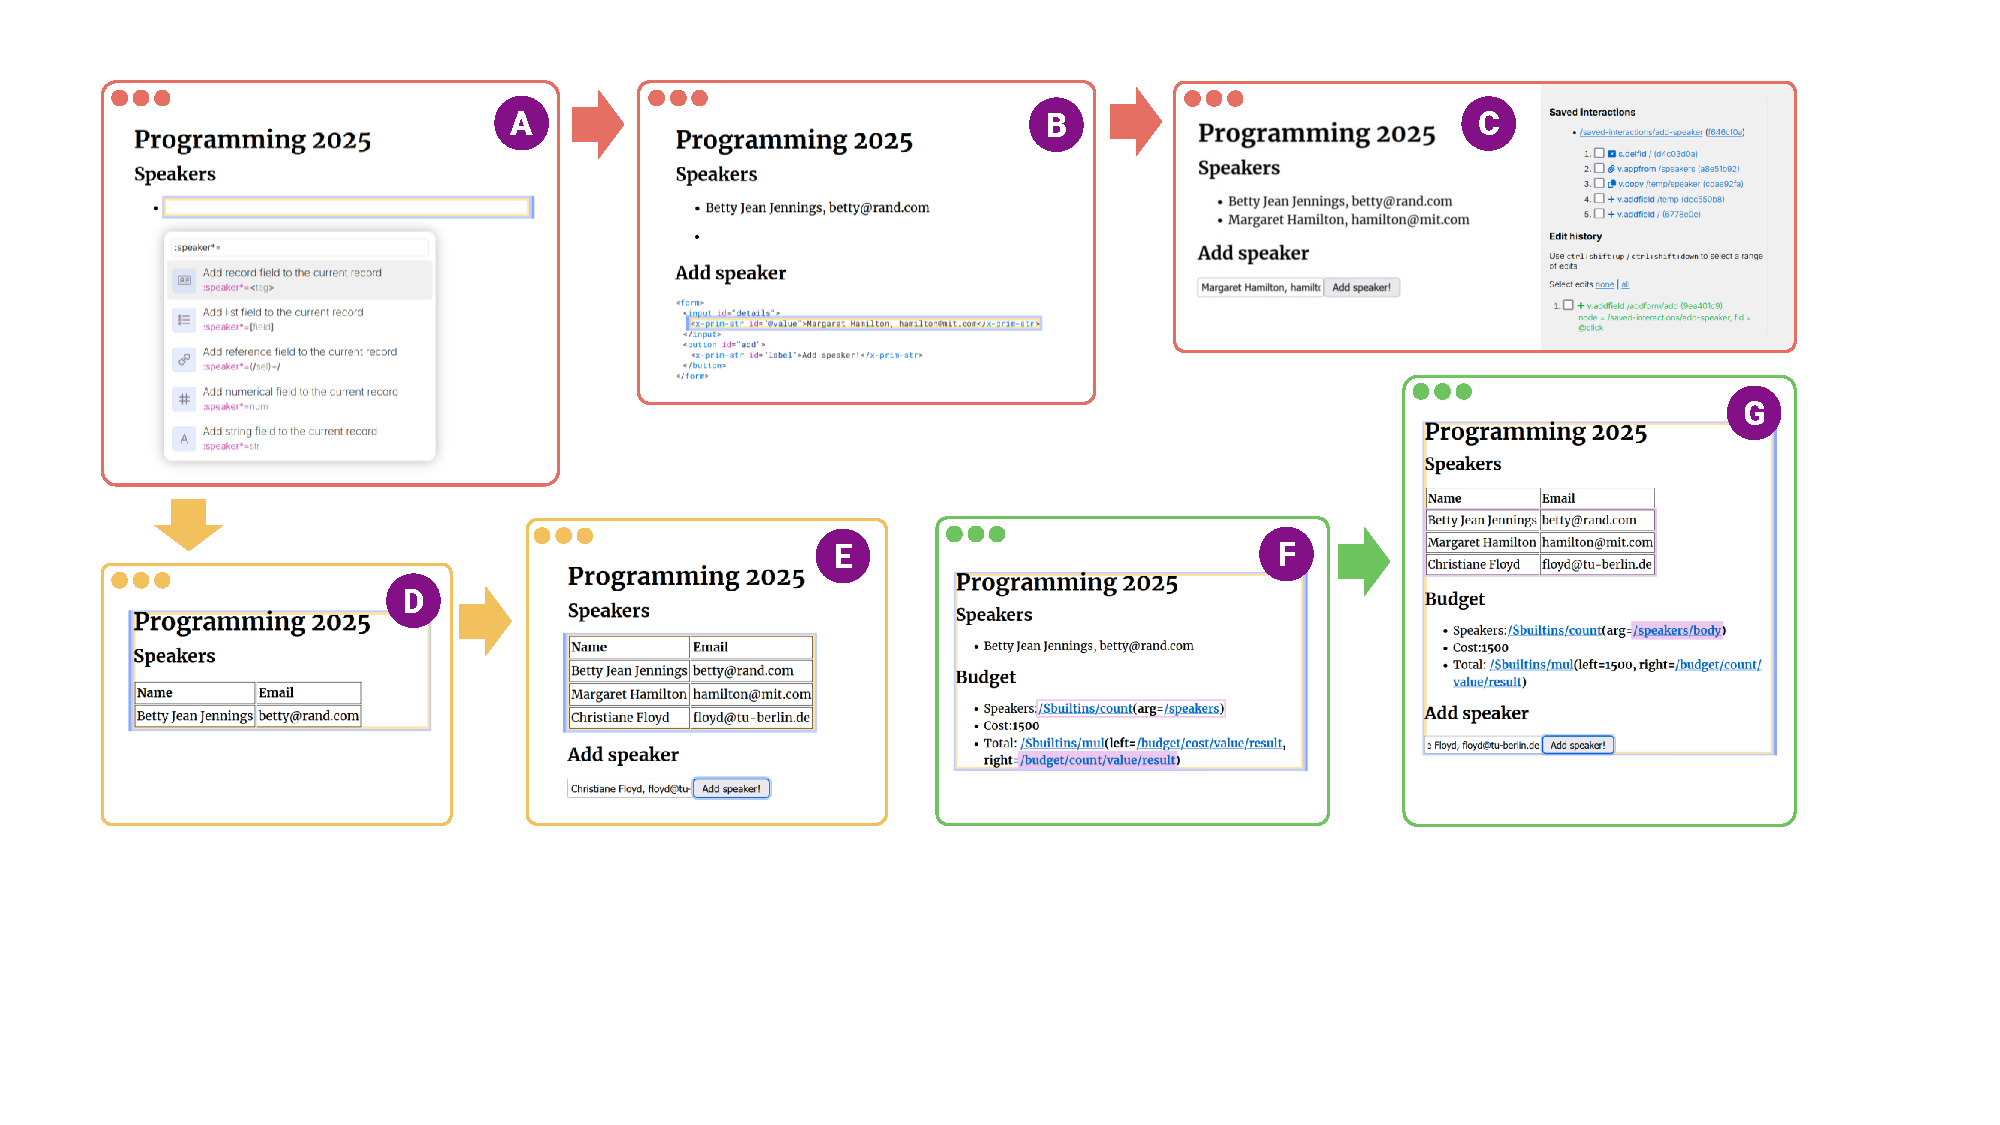
\includegraphics[width=0.95\textwidth,clip,trim=1cm 1cm 1cm 0.5cm]{fig/walkthrough.pdf}
\vspace{-1em}
\caption{Organizing a conference using Denicek. The Walkthrough shows construction of a user
  interface for adding speakers (A, B, C); refactoring of the list and merging edits (D, E); and
  formulas with schema and code co-evolution (F, G).}
\label{fig:walkthrough}
\end{figure*}

\newpage

% ==================================================================================================

\section{Walkthrough}
\label{sec:walk}

In this section, we use the web-based prototype Webnicek to illustrate programming
experiences enabled by the Denicek substrate (\S\ref{sec:impl}). Webnicek is based on a structure
editor that supports navigation in the document and issuing of edit commands. We follow two
formative examples (\S\ref{app:examples}) related to conference planning.

\subsubsection*{\circled{A} Adding a Speaker}
The user starts with an empty document, which is represented as a record. They add a field for
each heading and a list {\small\Verb_<ul>_}, represented by a field named {\small\Verb_speakers_}. They use the command
toolbox to add the first speaker.

\subsubsection*{\circled{B} Creating a User Interface} To simplify adding of
further speakers, the user creates a textbox and a button. They enter new speaker
details, add a new {\small\Verb_<li>_} element to the list and copy the speaker details
from the textbox into the new element using source view.

\subsubsection*{\circled{C} Saving the Interaction} After adding the speaker from the textbox,
the user opens history view, selects edits that added the speaker and saves those as the
{\small\Verb_add-speaker_} interaction. They attach this as a handler for the {\small\Verb_click_} event of the button.

\keyideabox{\faLightbulbO}{Programming by Demonstration}{Denicek implements programming by
demonstration (\S\ref{sec:impl-pbd}) by letting the user to save and replay past interactions,
either directly or by attaching them to a UI event.}

\subsubsection*{\circled{D} Refactoring Document Structure} Another user starts with the initial
version of the document and turns the list into a table. This is done by invoking a series of
commands that change tags, wrap elements, copy and transform values.

\subsubsection*{\circled{E} Merging Edits} The two document versions can be automatically merged.
The refactoring is applied to all existing speakers. New speakers added using the ``Add speaker!''
button are also automatically added in the new format.

\keyideabox{\faLightbulbO}{Local-First Collaboration}{Denicek's merging
reapplies edits from another branch on top of the current history (\S\ref{sec:impl-collab}).
Merging is asymmetic, but the order does not matter in the above scenario. The same merging
operation is used when handling user interaction (\S\ref{sec:impl-interaction}).}

\subsubsection*{\circled{F} Adding Budget Calculation} A third user adds budget calculation to
the initial document. Formulas are represented as special {\small\Verb_x-formula_} nodes whose arguments
are other nodes or references to other nodes or formulas (highlighted on mouse hover).

\keyideabox{\faLightbulbO}{Incremental Recomputation}{Evaluating a formula yields additional
edits that augment the document with the result. Those edits are kept
at the top of the document history and are removed in case of a conflict (\S\ref{sec:impl-incremental}),
providing incremental recomputation.}

\subsubsection*{\circled{G} Merging Formulas} When the budget calculation is merged with the
other edits, references in formulas are automatically updated to point to the new list.
Adding new speaker via the ``Add speaker!'' button invalidates the evaluated result.

\keyideabox{\faLightbulbO}{Schema Change Control}{The substrate understands references in
the document and updates them when applying structural edits (\S\ref{sec:impl-schema}).
Evaluation can replace formulas with values, but also augment them to enable
end-user debugging via provenance analysis (\S\ref{sec:impl-provenance}).}

% --------------------------------------------------------------------------------------------------

\arrayrulecolor{lightgray}
\definecolor{ekgray}{gray}{0.90}

\begin{figure}
\newcommand{\seltablecol}[3]{
\sffamily\small{\bfseries #2} & {\footnotesize #1} & \footnotesize #3\\
}
\newcommand{\ndtablecol}[4]{
\raisebox{-0.2em}{#1} & \sffamily\small{\bfseries #2}\,\;\textit{\footnotesize #3}\\[-0.2em]
&\sffamily\footnotesize #4\\[0.3em]
}

\begin{tabular}{|llp{18.08em}|}
\hline
\rowcolor{ekgray}
&&\\[-1em]
\rowcolor{ekgray}
\sffamily\small{\bfseries Selector} & {\sffamily\footnotesize Notation} & \\[0.2em]
\hline
&&\\[-1em]
\seltablecol{\Verb|..|}{Parent}{Refers to a parent of a node}
\seltablecol{\Verb|field|}{Field}{Refers to record field of a given name}
\seltablecol{\Verb|\#index|}{Index}{Refers to list element at a given index}
\seltablecol{\Verb|*|}{Any}{Refers to all children of a list node}
\hline
\end{tabular}

~\\[0.5em]

\begin{tabular}{|cl|}
\hline
\rowcolor{ekgray}
&\\[-1em]
\rowcolor{ekgray}
& \sffamily\small{\bfseries Kind}\;\,\textit{\footnotesize arguments} \\[0.2em]
\hline
&\\[-1em]
\ndtablecol{\faListUl}{List}{tag, index$_1$, child$_1$, $\ldots$, index$_n$, child$_n$}
  {Ordered list of nodes, addressable by \textit{index}. Renders as \Verb|<tag>| with children.}
\ndtablecol{\faFileO}{Record}{tag, field$_1$, child$_1$, $\ldots$, field$_n$, child$_n$}
  {Record with children addressable by \textit{field}. Renders as \Verb|<tag>| with children.}
\ndtablecol{\faExternalLink}{Reference}{selectors}
  {Reference to another document location. Displays the \Verb|selectors| as a link.}
\ndtablecol{\faFont}{Primitivie}{string \textnormal{or} number}
  {Numerical or textual primitive value. Renders as an HTML text node.}
\hline
\end{tabular}
\vspace{-0.5em}
\caption{Structure of selectors and document nodes}
\label{fig:doc}
\vspace{-1em}
\end{figure}

% ==================================================================================================

\section{The Denicek Substrate}
\label{sec:system}
Denicek represents programs as sequences of edits that construct and transform a computational
document. In this section, we describe the structure of documents and edits, as well as the
operations that form the backbone of the system and are used to implement the
end-user programming experiences discussed in \S\ref{sec:impl}.

% --------------------------------------------------------------------------------------------------

\subsection{Selectors, Documents and Edits}
A computational document is a tree, consisting of four kinds of nodes (Fig.~\ref{fig:doc}).
References to document locations can be relative or absolute. Both kinds can appear in a
document (reference nodes); absolute references are used in edits (to denote a target~node).

A reference is represented as a sequence of selectors (Fig.~\ref{fig:doc}).
The document model assumes that lists are homogeneous and records heterogeneous, and so the
\ident{Any} selector makes it possible to refer to all children of a list, but there is no
way to refer to all children of a record. Note that Denicek does not use implicit numerical
indices for lists. The index of a new item has to be supplied explicitly. The reasoning behind
this design choice is discussed in \S\ref{sec:discuss}.

\subsubsection*{Document Edits}
The supported document edits and their behavior are listed in Fig.~\ref{fig:edits}. All edits
require \emph{target} to which they are applied. Target is an absolute reference not containing the
\ident{Parent} selector. It can contain the \ident{Any} selector, in which case the edit is applied
to multiple nodes simultaneously. Most edits can only be applied to target node(s) of a specified
kind. As discussed in \S\ref{sec:discuss}, both fields of a record and list elements are ordered
and edits that add a new item take the index or field name of a previous node.

The edits allow any transformation of a document through a series of steps whose effect can be
tracked by the substrate. As we saw, Denicek updates references when document structure changes.
Fig.~\ref{fig:edits} distinguishes between edits that keep references in a document unchanged
(above) and edits that affect references (below).

Renaming a field or wrapping a node require corresponding change to references in the document
(\S\ref{sec:system-ops}). When deleting a field to which there is a reference in the document, Denicek
rejects the edit. A copy edit can also be rejected, because it is ambiguous whether references
referring to the original location should continue referring to the source or should be changed to
point to the target of the copying (a reference cannot refer to two locations).

% --------------------------------------------------------------------------------------------------

\begin{figure}
\newcommand{\ektablecol}[5]{
\raisebox{-0.2em}{#1} & \sffamily\small{\bfseries #2}\,\;\textit{\footnotesize target, #3} & \sffamily\footnotesize #4 \\[-0.2em]
&\multicolumn{2}{l|}{\sffamily\footnotesize #5}\\[0.3em]
}
\begin{tabular}{|cp{16em}r|}
\hline
\rowcolor{ekgray}
&&\\[-1em]
\rowcolor{ekgray}
 & \sffamily\small{\bfseries Edit}\;\,\textit{\footnotesize arguments} & \sffamily\footnotesize\bfseries Target \\[0.2em]
\hline
&&\\[-1em]
\ektablecol{\faPlus}{Add}{field, after, node}{Record}
  {Add \textit{node} as a \textit{field} to the specified record \textit{after} a given field.}
\ektablecol{\faAt}{Append}{index, after, node}{List}
  {Append \textit{node} to the end of the specified list \textit{after} a given field.}
\ektablecol{\faSort}{Reorder}{permutation}{List}
  {Reorder items of a specified list according to a \textit{permutation}.}
\ektablecol{\faMinusCircle}{DeleteItem}{index}{List}
  {Delete the item at a given \textit{index} of a specified list.}
\ektablecol{\faCode}{UpdateTag}{tag}{List or Record}
  {Change the tag of a specified list or record from to a new \textit{tag}.}
\ektablecol{\faICursor}{PrimitiveEdit}{transform}{Primitive}
  {Apply primitive \textit{transform} to the specified primitive.}
\hline
&&\\[-1em]
\ektablecol{\faFont}{RenameField}{old field, new field}{Record}
  {Rename the field of a specified record from \textit{old} to \textit{new}.}
\ektablecol{\faTimesCircle}{DeleteField}{field}{Record}
  {Delete the field \textit{field} of a specified record.}
\ektablecol{\faFileO}{WrapRecord}{tag, field}{Any}
  {Wrap the specified node as a \textit{field} of a new record with \textit{tag}.}
\ektablecol{\faListUl}{WrapList}{tag, index}{Any}
  {Wrap the specified node as a sole element of a new list with \textit{tag}.}
\ektablecol{\faCopy}{Copy}{selectors}{Any}
  {Copy nodes(s) from \textit{selectors}, replacing the specified target(s). }
\hline
\end{tabular}
\vspace{-0.5em}
\caption{Summary of document edit types in Denicek}
\label{fig:edits}
\vspace{-1em}
\end{figure}

% --------------------------------------------------------------------------------------------------

\subsubsection*{Automatic Reference Update}
There are two situations in which automatic update of references is undesirable. If an edit is
applied to a singular element of a list (reference contains the \ident{Index} selector),
references that refer into the list should be unchanged. Although such edits violate the invariant
that collections are homogeneous, they typically do so only temporarily, for example during
construction of a new list item (checking such edits is discussed in \S\ref{sec:discuss-future}).

Documents can also contain values that can be of multiple different kinds (i.e., a union type).
In such case, references should not be updated when the kind of the value changes. For example,
a formula may be either unevaluated or evaluated. As discussed in \S\ref{sec:impl-eval}, evaluation
involves wrapping the formula node, but this should not affect references to the formula.
To support those cases, edits that normally affect selectors (Fig.~\ref{fig:edits}, below)
have a \emph{reference behavior} field that can be set to disable automatic reference
updating. This annotation is required when the target contains the \emph{Index} selector.

\subsubsection*{No Conditional Edits.}
An important aspect of the design is that the effect an edit has on references inside
the document does not depend on the current value of the document. This makes it possible to
define merging solely in terms of edits, without reference to current document state.
(The effect \ident{Copy} has on the document structure depends on the existing document
structure, but not on its value).

This design choice makes it impossible to encode computational logic directly in the edits
(e.g., through conditional edits). As we will see in \S\ref{sec:impl-interaction}, such logic
can be provided as an additional mechanism on top of the underlying Denicek substrate.

% --------------------------------------------------------------------------------------------------

\subsection{Primitive Operations}
\label{sec:system-ops}
Denicek provides three primitive operations. A sequence of edits can be applied to a document, two
sequences of edits can be merged and also checked for conflicts. Denicek identifies edit histories by
a (git-like) hash, computed from the hash of the parent and the current edit. The hash is used to
identify a common shared part of the history during conflict resolution and merging.

\subsubsection*{Applying Edits}
When applying an edit, Denicek locates the target node and transform it according to the edit. If
the edit can affect references in the document (Fig~\ref{fig:edits}, below), Denicek updates
matching references in the document according to the rules shown in Fig.~\ref{fig:updates} provided
that the reference behavior of the edit is not set to disable the updating (this is required when
the target reference contains the \ident{Index} selector). Reference update behavior for
\ident{WrapRecord} and \ident{WrapList} differs in that the updated references as a result of
\ident{WrapList} use the \ident{All} selector. Although \ident{WrapList} specifies the index to
be used for the newly created list item, we assume that the operation introduces a homogeneous
list and the new reference should point to all eventual list items.

Also note that affected references in the document may be more specific than the edit
target. For example, if we rename {\small\Verb|old|} to {\small\Verb|new|} at {\small\Verb|/foo/*|},
a reference {\small\Verb|/foo/3/old|} will become {\small\Verb|/foo/3/new|}. (A reference in the
document cannot be more general, because such edit would have to contain the \ident{Index} selector
and this would require setting reference behavior to not trigger reference update.) Finally,
if the document contains a reference that would be invalidated by the \ident{Copy} or
\ident{DeleteField} edit, the edit is rejected.

\subsubsection*{Merging Edit Histories}
Merging edit histories is used when two users edit document independently, but also
when replaying edits in programming by demonstration. The
operation works on two edit histories, $E, E_1$ and $E, E_2$, that have a shared prefix $E$.
The merging operation is akin to git rebase. It turns edits $E_2$ into edits $E_2'$ that
can be reapplied on top of the other edit history, resulting in a new history $E, E_1, E_2'$.
Note that the operation is not symmetric. If there are conflicts among the edits in $E_1$ and
$E_2$, the result of $E, E_1, E_2'$ will differ from the result of $E, E_2, E_1'$.
We return to this problem in the next section when discussing conflict detection.

The key operation that enables such reconcilliation takes two individual edits that occurred
indpendently, $e_1$ and $e_2$, and produces a sequence of edits $e_2', e_2'', \ldots$ that
can be applied after $e_1$ and have the effect of $e_2$, modified to respect the effects of $e_1$.
There are two aspects of such reconcilliation:

\begin{enumerate}
\item \emph{Apply to Newly Added.} If $e_2$ is adding new nodes to the document, but
  $e_1$ modified the document through a selector that would also affect the new nodes added by $e_2$,
  we need to apply the transformation represented by $e_1$ to the nodes newly added by $e_2$.
  This is done by generating an additional edit, to be applied after $e_2$, that is based on
  $e_1$ but targets only the newly added nodes (more details can be found in \S\ref{app:merge-apply-to-added}).

\item \emph{Transform Matching References.} If $e_2$ targets a node that is inside a node
  whose structure is changed by $e_1$, the target reference in $e_2$ is updated in a way that
  corresponds to the new structure. This is done using the rules shown in Fig.~\ref{fig:updates},
  that apply when transforming references inside a document, although we also support the case
  when $e1$ is \ident{Copy} (see \S\ref{app:merge-transform-refs} for details).
\end{enumerate}

% --------------------------------------------------------------------------------------------------

\begin{figure}
\newcommand{\tttablecol}[5]{
\small{\bfseries #1}\;\,\footnotesize\textit{#2}\,\; --\,\; #5\\[-0.1em]
\quad \footnotesize #3 \;\;$\Rightarrow$\;\; #4 \\[0.3em]
}
\begin{tabular}{|p{27em}|}
\hline
\\[-1em]
\tttablecol{RenameField}{target, old field, new field}{\Verb|/target/old\_field/nested|}{\Verb|/target/new\_field/nested|}
  {Replace Field for matching references.}
\tttablecol{WrapRecord}{target, tag, field}{\Verb|/target/nested|}{\Verb|/target/field/nested|}
  {Insert extra Field selector after matching prefix.}
\tttablecol{WrapList}{target, index, tag}{\Verb|/target/nested|}{\Verb|/target/*/nested|}
  {Insert extra All selector after matching prefix.}
\hline
\end{tabular}
\vspace{-0.5em}
\caption{How document edits transform references}
\label{fig:updates}
\vspace{-1em}
\end{figure}

% --------------------------------------------------------------------------------------------------

\begin{figure}
\newcommand{\eftablecol}[3]{
\small{\bfseries #1}\;\footnotesize\textit{target}\,\; --\,\; {\footnotesize #2}\\[-0.1em]
\quad \small #3\\[0.3em]
}
\begin{tabular}{|p{27em}|}
\hline
\\[-1em]
\eftablecol{StructureEffect}{Affects fields or structure of the target node.}
  {\ident{RenameField}, \ident{DeleteField}, \ident{WrapRecord}, \ident{WrapList}, \ident{Copy}}
\eftablecol{ValueEffect}{Transforms value, modifies list or adds an additional field.}
  {\ident{Add}, \ident{Append}, \ident{Reorder}, \ident{DeleteItem}, \ident{PrimitiveEdit}}
\eftablecol{TagEffect}{Modifies the tage of the target node.}
  {\ident{UpdateTag}}
\hline
\end{tabular}
\vspace{-0.5em}
\caption{Effects of individual edit operations}
\label{fig:effects}
\vspace{-1em}
\end{figure}

% --------------------------------------------------------------------------------------------------

To illustrate merging, consider a case where we created a list of work items {\small\Verb|/todo|}.
In one branch, we add an additional item to the list ($e_2$). In another branch, we wrap the
list in an extra \ident{<div>} element ($e_1$) and add a checkbox to each work item ($e_1'$):
%
\begin{equation*}
\arraycolsep=2pt
\begin{array}{rcl}
e_2 &=& \srckvd{Append}(\textnormal{\small\Verb|/todo|}, \#1, \#0, \srcid{<li>Do some work</li>})\\[0.5em]
e_1 &=& \srckvd{WrapRecord}(\textnormal{\small\Verb|/todo|}, \srcid{<div>}, \srcid{items})\\
e_1' &=& \srckvd{Add}(\textnormal{\small\Verb|/todo/items/*|}, \srcid{done}, \srckvd{nil}, \srcid{<input type="checkbox"/>})\\
\end{array}
\end{equation*}
%
If we want to append the edit $e_2$ after edits $e_1, e_1'$, we need to update its target to
reflect the additional wrapping (2) and we need to create and additional \ident{Add} operation
that will add the checkbox to the new item (1). The result is two edits $e_2', e_2''$:
%
\begin{equation*}
\arraycolsep=2pt
\begin{array}{rcl}
e_2'  &=& \srckvd{Append}(\textnormal{\small\Verb|/todo/items|}, \#1, \#0, \srcid{<li>Do some work</li>})\\
e_2'' &=& \srckvd{Add}(\textnormal{\small\Verb|/todo/items/\#1|}, \srcid{done}, \srckvd{nil}, \srcid{<input type="checkbox"/>})\\
\end{array}
\end{equation*}
%
If we performed the merge operation in the other order, we would simply append $e_1, e_1'$ after
$e_2$. Although this is not the case in general, the result will be the same regardless of the order here.

\subsubsection*{Conflict Resolution}
When merging two sequences of edits, $E, E_1$ and $E, E_2$, it is sometimes possible to construct
edit histories $E_1'$ and $E_2'$ such that the results of applying $E, E_1, E_2'$ and
$E, E_2, E_1'$ are the same. However, this is not always the case. Two edits can conflict if
they both modify the same value, if they transfrom the structure of a node in incompatible ways
or if one modifies a node nested inside a node replaced or deleted by the other.
Detected conflicts can be reported to the user, but we also use conflict detection to
implement incremental evaluation (\S\ref{sec:impl-incremental}).

The Denicek substrate implements a conflict detection mechanism inspired by effect
systems~\cite{lucassen-1988-effects}. The mechanism is simple and tractable, but over-approximates
conflicts, i.e.~it may report a conflict even if two edits can be merged successfully
(see \S\ref{sec:discuss-future}). An effects describe how an edit affects the document structure
and we distinguish between three types of effects as shown in Fig.~\ref{fig:effects}.

We say that a set of effects $F_1$ conflicts with another set of effects $F_2$ if there
are effects $f_1\in F_1$ and $f_2\in F_2$ such that they are of the same kind and the target
of $f_1$ is a prefix of the target of $f_2$ or vice versa (allowing specific \ident{Index} to
match against \ident{All} in any direction).

Given two edit histories $E, E_1$ and $E, E_2$, Denicek can use conflict detection to remove
all conflicting edits from $E_2$ and produce a sequence of remaining edits $e_2', e_2'', \ldots$
that can be added after $E, E_1$ and do not conflict with edits in $E_1$.

To do this, we iterate over edits $e_2$ from $E_2$ and check if the dependencies of $e_2$
conflict with effects of (1) any of the effect $e_1$ from $E_1$ or (2) effects of any of the
previously removed edits. Here, the dependencies of $e_2$ include its target, but also source
of \ident{Copy} and additional dependencies recorded explicitly as discussed in
\S\ref{sec:impl-incremental}. If a conflict is detected, the edit $e_2$ is removed and its effect
is recorded, so that we remove any subsequent edits that would depend on the removed edit.

% ==================================================================================================

\section{Programming Experiences Implementation}
\label{sec:impl}

The key claim of this paper is that the Denicek computational substrate
makes it easy to support a range of experiences that make programming more concrete,
collaborative and interactive.

In this section, we describe how Webnicek uses the substrate
to support local-first collaboration (\S\ref{sec:impl-collab}), programming by
demonstration (\S\ref{sec:impl-pbd}, \S\ref{sec:impl-interaction}), incremental recomputation
(\S\ref{sec:impl-eval}, \S\ref{sec:impl-incremental}), schema change control (\S\ref{sec:impl-schema}),
end-user debugging via provenance tracking (\S\ref{sec:impl-provenance})
and concrete programming via managed copy \& paste (\S\ref{sec:impl-copy}).

We describe the programming experience in isolation in this section. The next section provides a
more comprehensive evaluation through a case study that combines multiple of them together.

% --------------------------------------------------------------------------------------------------

\begin{figure}[t]
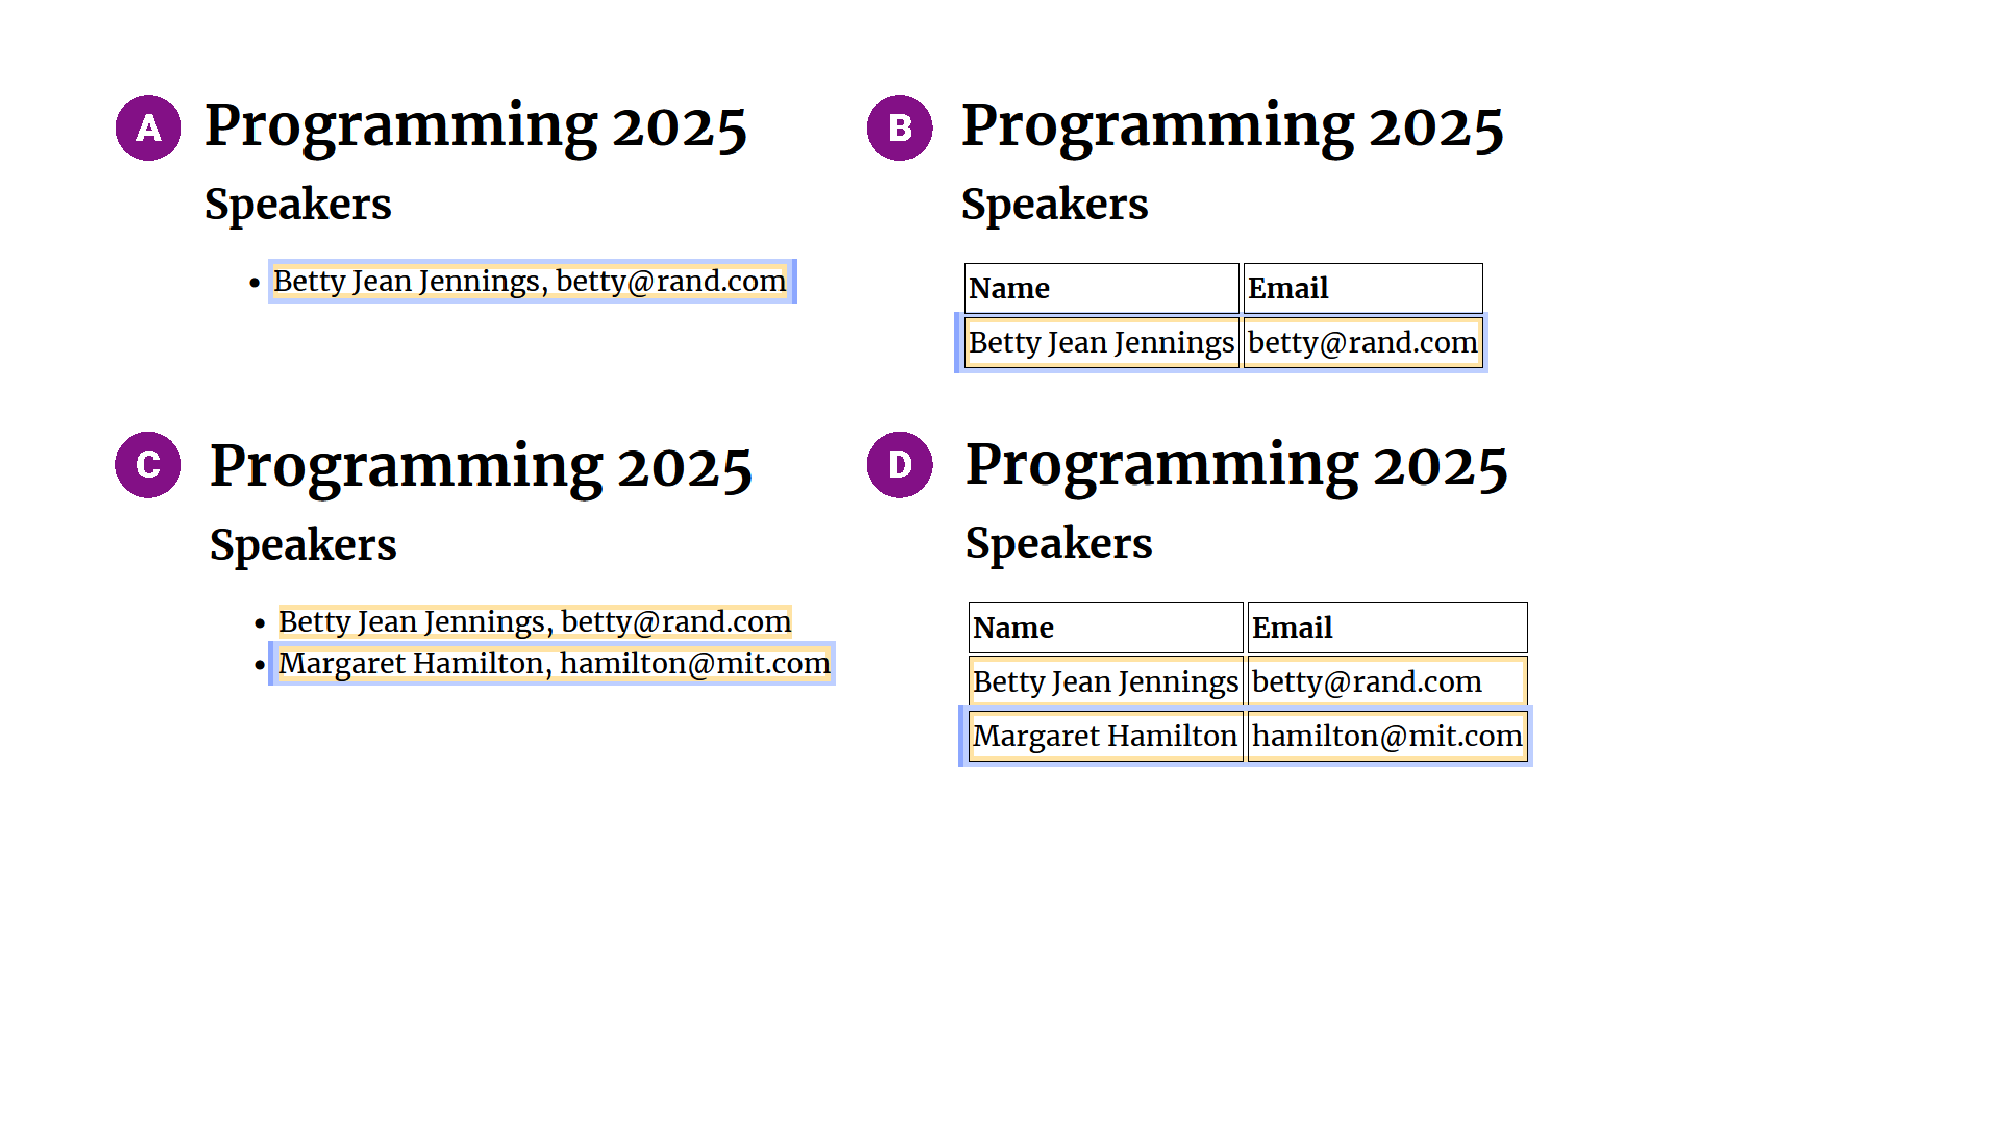
\includegraphics[width=0.9\columnwidth,clip,trim=1.7cm 6cm 7.8cm 1.5cm]{fig/merging.pdf}
\caption{Merging of two independently done sequences of edits. Two ways of merging B and C result in the same D.}
\label{fig:merging}
\end{figure}

% --------------------------------------------------------------------------------------------------

\subsection{Local-First Collaboratation}
\label{sec:impl-collab}

The Denicek representation enables local-first collaboration~\cite{kleppmann-2019-local},
as illustrated previously in \S\ref{sec:walk} (E). If a document is edited by multiple users, they can
each make edits to their local copy and eventually merge the variants using the operation to
merge edit histories.

Merging of histories behaves akin to git rebase in that it keeps a linear history. Synchronization
in a distributed system thus requires first reapplying local edits on top of the remote history,
before updating the remote history. Denicek thus implements the \emph{convergence model} of
document variants \cite{edwards-2025-schema}, i.e., the user cannot, for example, maintain their
own local document structure and import new data from another variant (an alternative discussed
in \S\ref{sec:discuss}).

Recall that merging of edit histories is not symmetric. Document $D$ in Fig.~\ref{fig:merging}
can be obtained either by appending $C'$ (produced by the edit reconcilliation operation)
on top of $A,B$ or by appending $B'$ on top of $A,C$. According to our effect analysis, the two
operations are conflicting. Although $B$ primarily affects the document structure, it also adds
a new field to the record (email), which is a \ident{ValueEffect}, conflicting with
\ident{ValueEffect} of $C$. In this scenario, the conflict can be ignored and the resulting document
is the same in both cases.

However, the resulting two histories will differ. In the first case, the
\ident{Append} edit that adds a new node is supplemented by further focused edits that transform
the added node from a list item to a new table row.
In the second case, the structural transformations are automatically applied to all rows.
As discussed in \S\ref{sec:system-ops}, conflicts during merging can be resolved either by
removing conflicting edits or by letting the later edits overwrite the former ones.

% --------------------------------------------------------------------------------------------------

\begin{figure}[t]
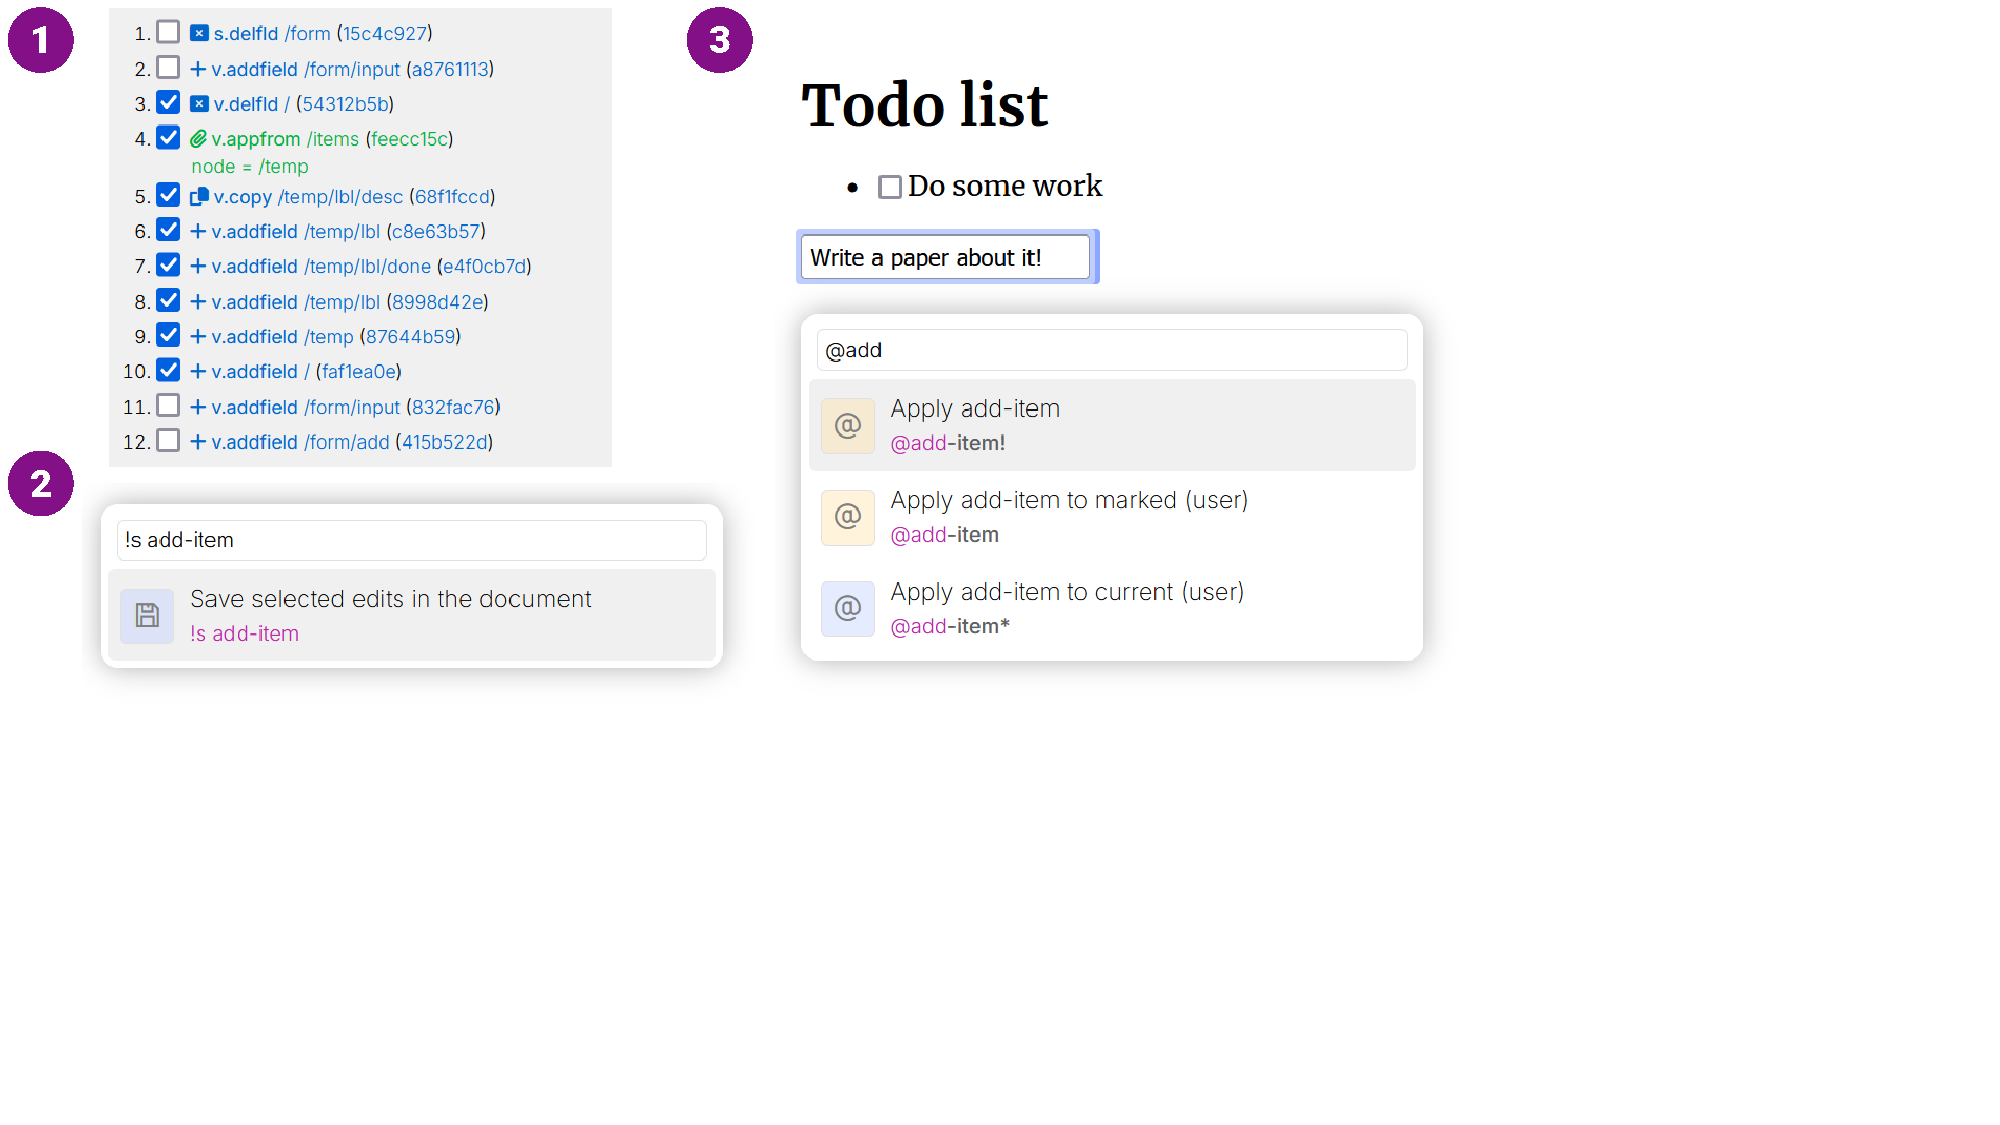
\includegraphics[width=0.9\columnwidth,clip,trim=0cm 7cm 9cm 0cm]{fig/pbd.pdf}
\caption{Programming by demonstration is implemented by selecting edits from the document
history (1), saving them in the document (2) and replaying them (3).}
\label{fig:pbd}
\end{figure}

% --------------------------------------------------------------------------------------------------

\subsection{Programming By Demonstration}
\label{sec:impl-pbd}

In programming by demonstration \cite{cypher-1993-pbd}, the user demonstrates a task to the
system and the system then repeats it, directly or in a generalized way. To use direct
repetition with Denicek (Fig.~\ref{fig:pbd}), the user can select edits from the edit history,
name them and replay them. In case of general-purpose document editing in Webnicek, this requires
certain forethought, but as illustrated in \S\ref{sec:case}, the mechanism is very effective in
a domain such as data wrangling \cite{kandel-2011-wrangler}.

There are two notable aspects of our implementation of programming by demonstration in Webnicek.
First, Webnicek records edits in the document itself (by representing individual edits as nodes and
storing them in list inside a {\small\Verb_/saved-interactions_} field). This means that no other
implementation mechanism outside of the system is needed and also that the stored edits can be
modified by the user or tools working with the document.

Second, to replay edits, Webniceks does not append the recorded edits on top of the current history.
When saving edits, it stores the hash of the history at the time of saving. When replaying,
it appends the recorded edits to the top of the original history (at the time of saving) and merges
this new sequence of edits with the current history. This pushes the recorded edits through all
subsequent edits made by the user. The result can be seen in Fig.~\ref{fig:walkthrough} (E), where
a newly added speaker is transformed from a list item to a table row.

Webnicek also accounts for the case where edits recorded in the document are themselves
transformed (when they are reconcilliated with other edits during merging). In this case, Webnicek
updates the recorded edits (an alternative approach is discussed in \S\ref{sec:discuss}).

% --------------------------------------------------------------------------------------------------

\begin{figure}[t]
\vspace{-0.5em}
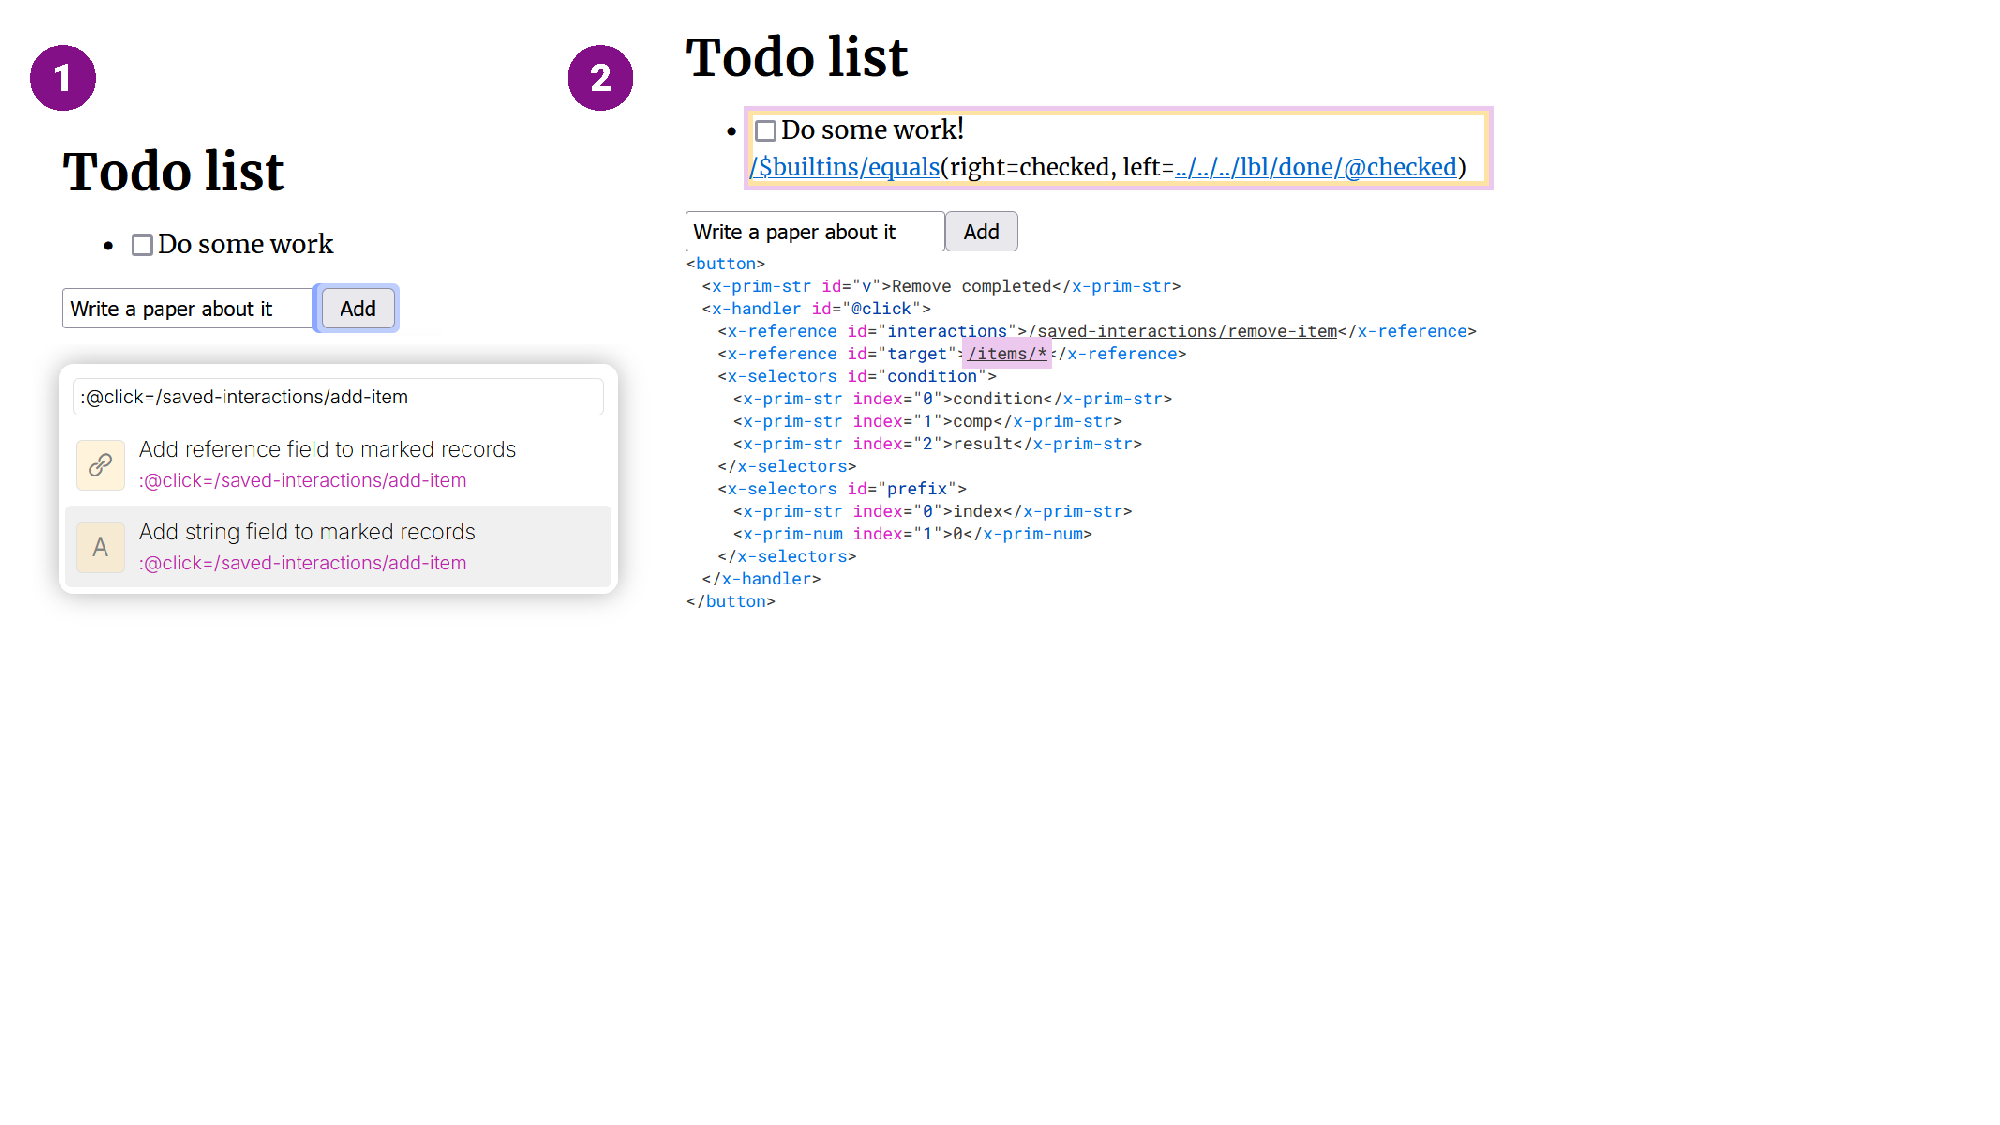
\includegraphics[width=1\columnwidth,clip,trim=0.5cm 8.5cm 8.5cm 0.5cm]{fig/interactive.pdf}
\vspace{-1.25em}
\caption{Using programming by demonstration to define a UI. The ``Add'' button (1) replays edits;
the ``Remove completed'' button (2) modifies target and specifies a condition. }
\label{fig:interactive}
\vspace{-1em}
\end{figure}

% --------------------------------------------------------------------------------------------------

\subsection{Interactive User Interfaces}
\label{sec:impl-interaction}

Programming by demonstration can be used to define interactive elements in the document. In a
simple scenario, illustrated in Fig.~\ref{fig:interactive}~(1), the {\small\Verb_click_} event
handler is set to a reference to a sequence of edits recorded in the document. Clicking the button
executes the edits using the mechanism discussed in \S\ref{sec:impl-pbd}, i.e., Webnicek appends
the edits to a history at the time when the edits were recorded and merges the edits with the
current history.

The use of merging when replaying recorded edits is crucial in both the Todo App example and the
Conference List example (see \S\ref{app:examples}). In both cases, it makes it possible to define
a user interface for adding items (new Todo items, new speakers) and later change the document
structure (refactor speaker list to a table) or add functionality (formula to evaluate whether a
Todo item has been completed) without having to recreate the user interface for adding items.
The use of merging ensures that new items are added in a correct format or with the additional
functionality.

Denicek can be used to generalize the interactions recorded through programming by
demonstration. Our prototype illustrates this option in a limited way. As shown in
Fig.~\ref{fig:interactive}~(2), a button to remove all completed Todo items can be created by
generalising the {\small\Verb_remove-item_} interaction, which removes the list item at the index 0.
In addition to the recorded interaction, we manually specify (in the source view) that the edits
should be applied to all elements selected by the {\small\Verb_/items/*_} selector, instead of
the original {\small\Verb_/items/0_} selector (prefix) and that the edits should only be
applied to elements for which the formula (which tests if the checkbox is checked) specified by a
relative selector {\small\Verb_./condition/comp/result_} evaluates to true.

\keyideabox{\faMagic}{Generalization Heuristic}{Specifying generalization manually is cumbersome.
Programming by demonstration systems typically implement heuristic for generalization
\cite{myers-2000-intelligence} infers and suggests such generalizations. If integrated into
a system based on Webnicek, such heuristic could automatically construct a formula
based on positive and negative examples \cite{gulwani-2014-flash} (selected and deselected items).}

% --------------------------------------------------------------------------------------------------

\subsection{Formula Language and Evaluation}
\label{sec:impl-eval}

Denicek documents can contain formulas inspired by the spreadsheet
paradigm \cite{nardi-1990-spreadsheets}. Formulas can specify richer computations than
what can be expressed using document edits. Formulas do not transform the document and their
results are transient, although their evaluation also leverages the substrate operations,
namely merging of edit histories.

As illustrated in Fig.~\ref{fig:counter}, formulas are represented as document nodes with a
special tag ({\small\Verb_<x-formula>_}). They are recognized by a formula evaluator and
rendered in a special way (\circled{1} and \circled{4}), but they are created using ordinary
edits and the Denicek substrate treates them as stnadard nodes.

To evalaute formulas, the formula evaluator generates edits that turn the {\small\Verb_<x-formula>_}
record into {\small\Verb_<x-evaluated>_} (\circled{2} and \circled{3}), which keeps the previous
formula state in the {\small\Verb_formula_} field and the evaluation result in the {\small\Verb_result_} field.
(Keeping the previous state of the formula is not necessary, but it enables provenance analysis
as discussed in \S\ref{sec:impl-provenance}.) The way edits generated by evaluation are merged
with the document is discussed in the next section.

The Counter App example shown in Fig.~\ref{fig:counter} illustrates the interaction between formulas
and programming by demonstration. To implement a counter, the Increment and Decrement buttons
wrap the current counter value in a formula that adds or subtracts 1.

\keyideabox{\faSuperscript}{Formula Language}{
Webnicek exposes the underlying representation of formulas to the user, but the same representation
can be edited through a user-friendly mechanism such as a block-based editor
\cite{jansen-2019-xlblocks} or a calculation view \cite{sarkar-2018-calc}. The key point
is that Denicek's tree structure makes it easy to embed formulas in document in a uniform
way, edit them and merge them with other changes.}

% --------------------------------------------------------------------------------------------------

\begin{figure}[t]
\vspace{-0.5em}
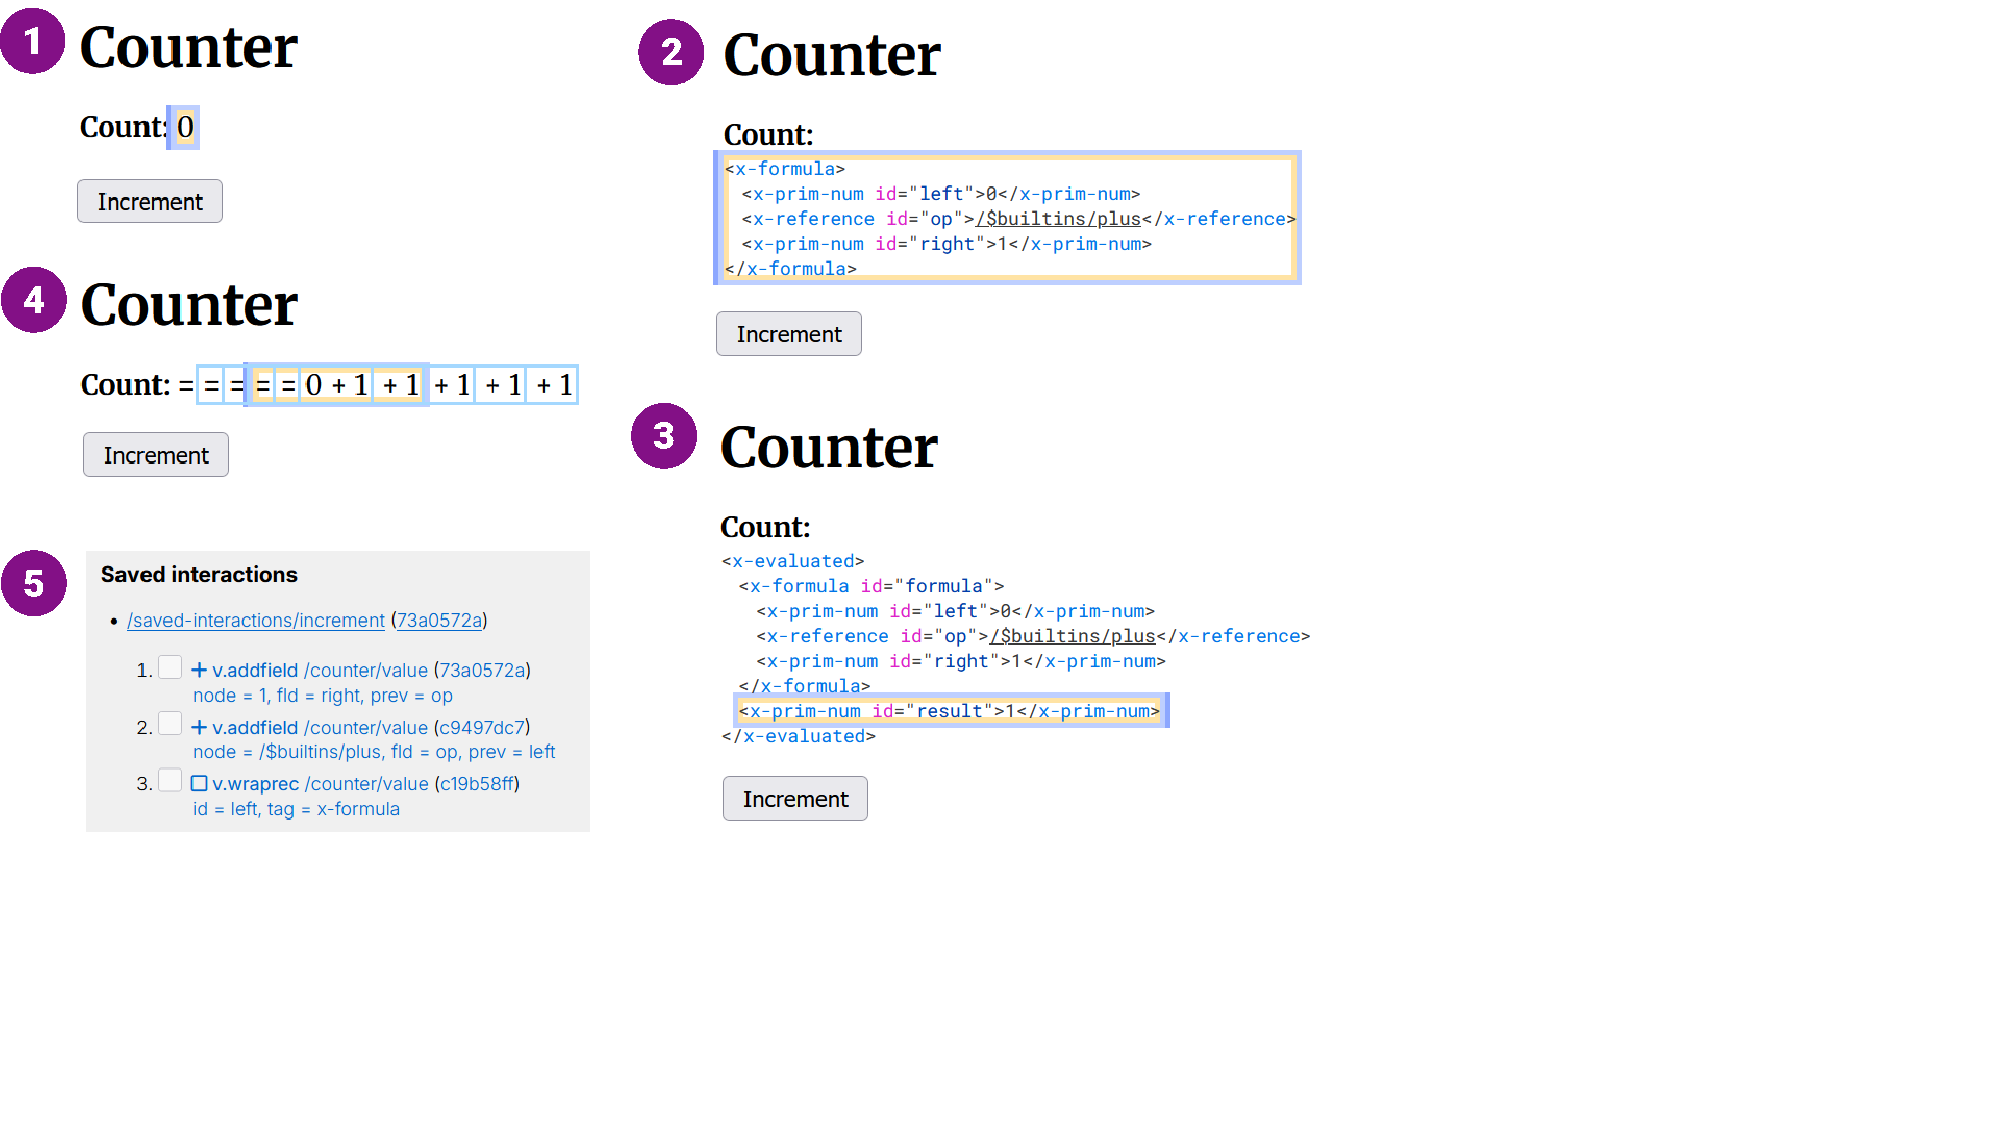
\includegraphics[width=0.95\columnwidth,clip,trim=0cm 7cm 8cm 0cm]{fig/counter.pdf}
\vspace{-0.5em}
\caption{Increment wraps the existing count in a formula that adds 1 to the
previous value (1), (2). Evaluation produces the count (3), which is invalidated on subsequent clicks (4).}
\label{fig:counter}
\vspace{-1em}
\end{figure}

% --------------------------------------------------------------------------------------------------

\begin{figure}[t]
\centering
\vspace{-0.5em}
\begin{minipage}{0.55\columnwidth}
  ~\\[1em]
  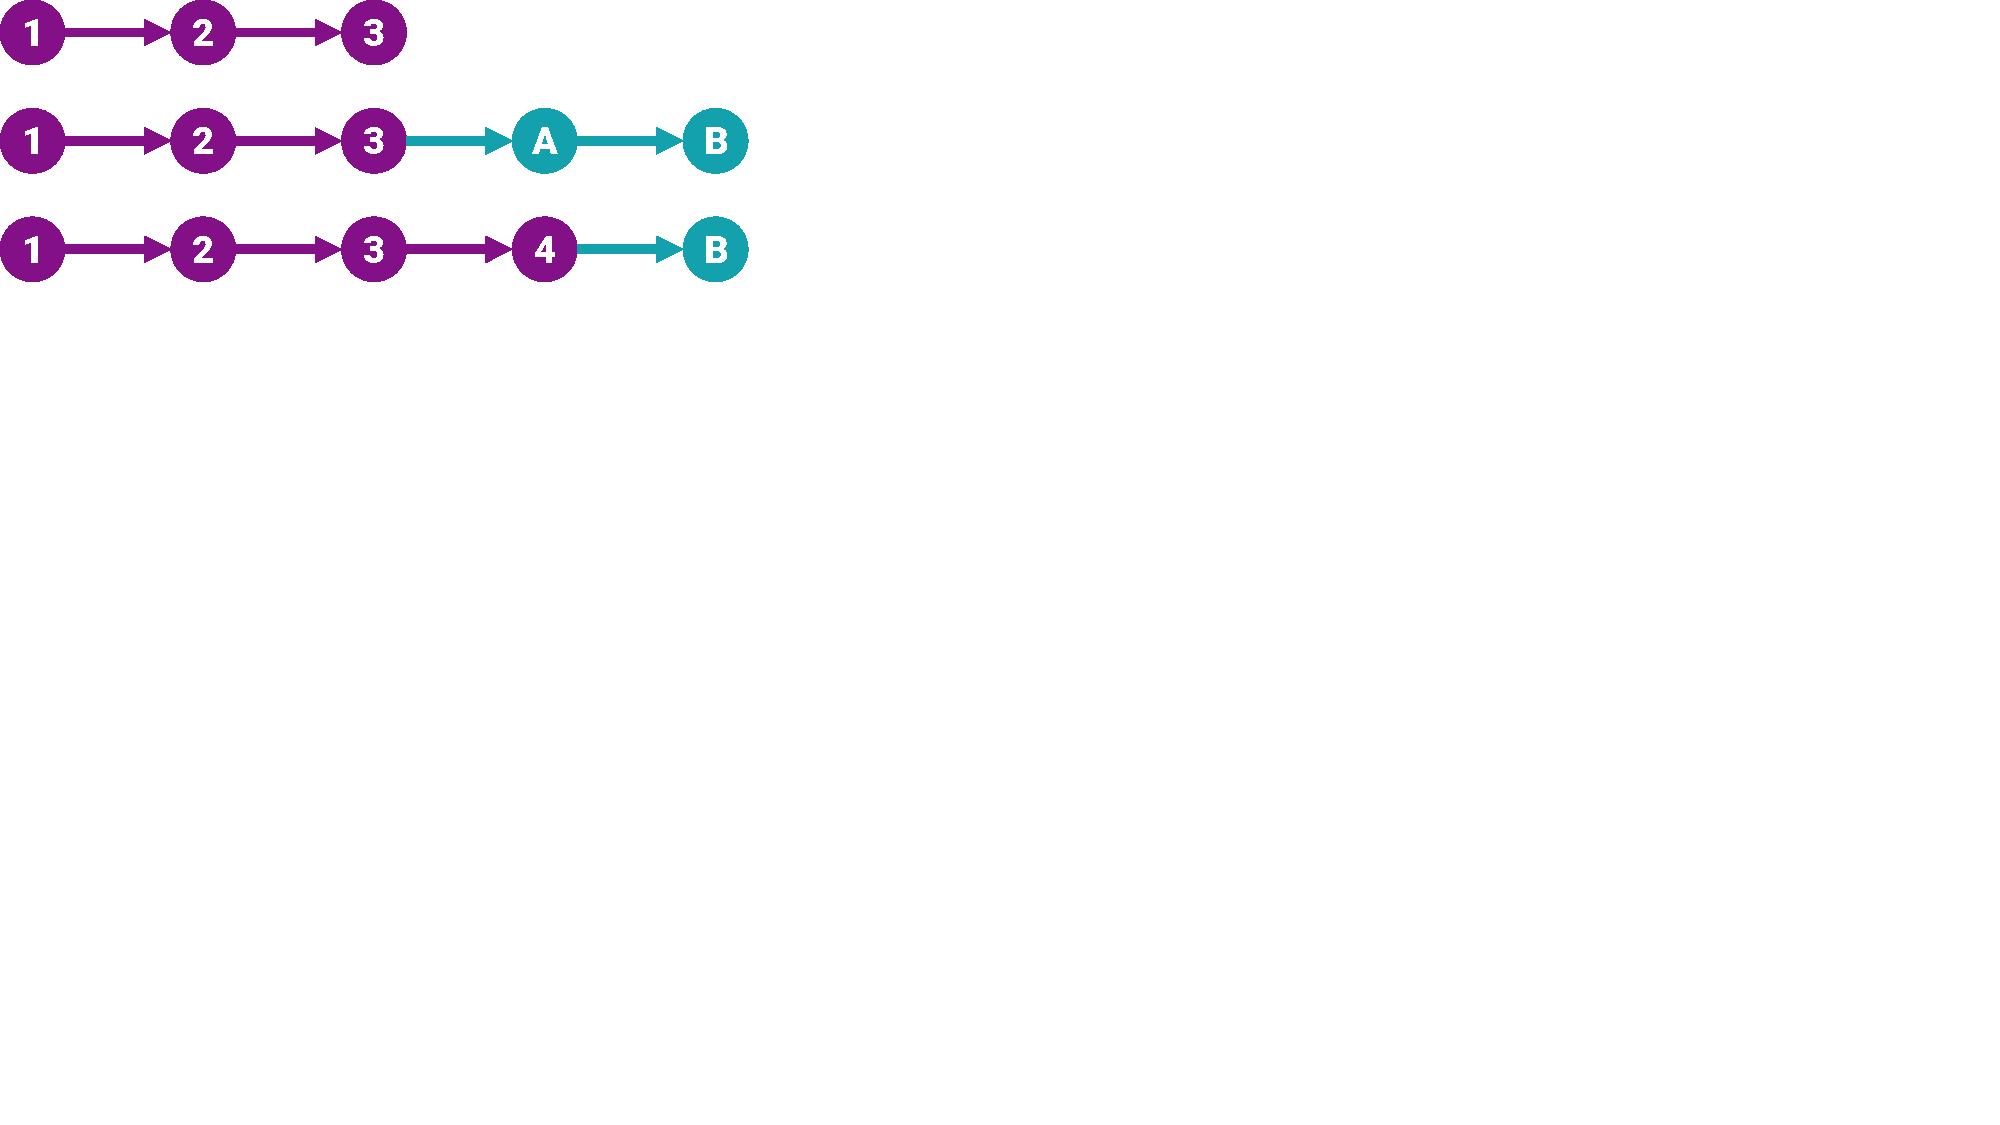
\includegraphics[width=0.9\columnwidth,clip,trim=0cm 14cm 21cm 0cm]{fig/eval.pdf}
  \end{minipage}%
  \begin{minipage}{0.45\columnwidth}
    \caption{Evaluated edits (A, B) are kept at the top of the history. When they conflict with
    ordinary edits (4), they are removed (A).}
    \label{fig:eval}
  \end{minipage}
  \vspace{-1em}
\end{figure}

% --------------------------------------------------------------------------------------------------

\subsection{Incremental Recomputation}
\label{sec:impl-incremental}

As illustrated in Fig.~\ref{fig:incremental}, Webnicek supports incremental re-computa\-tion.
In the example, the cost of speaker travel depends on the number of speakers, but the cost
of refreshments depends only on two constants. Edit that adds a speaker only invalidates the
former.

The evaluation mechanism is illustrated in Fig.~\ref{fig:eval}. When the formulas are evaluated,
Webnicek generates \emph{evaluated edits} that are appended to the top of the history.
When subsequent edits are made, they are appended after all non-evaluated edits and the
evaluated edits are pushed through the newly added edits. If the edits conflict (according to
conflict detection discussed in \S\ref{sec:system-ops}), affected evaluated edits and edits that
depend on them are dropped.

\keyideabox{\faRefresh}{Live Programming}{The Webnicek prototype does not automatically
evaluate formulas. This makes it easier to understand the evaluation
mechanism, but a realistic system based on the substrate could automatically evaluate
formulas to provide a live programming experience \cite{petricek-2020-foundations,rein-2019-live}
and use incremental recomputation for performance~reasons.}

% --------------------------------------------------------------------------------------------------

\begin{figure}[t]
  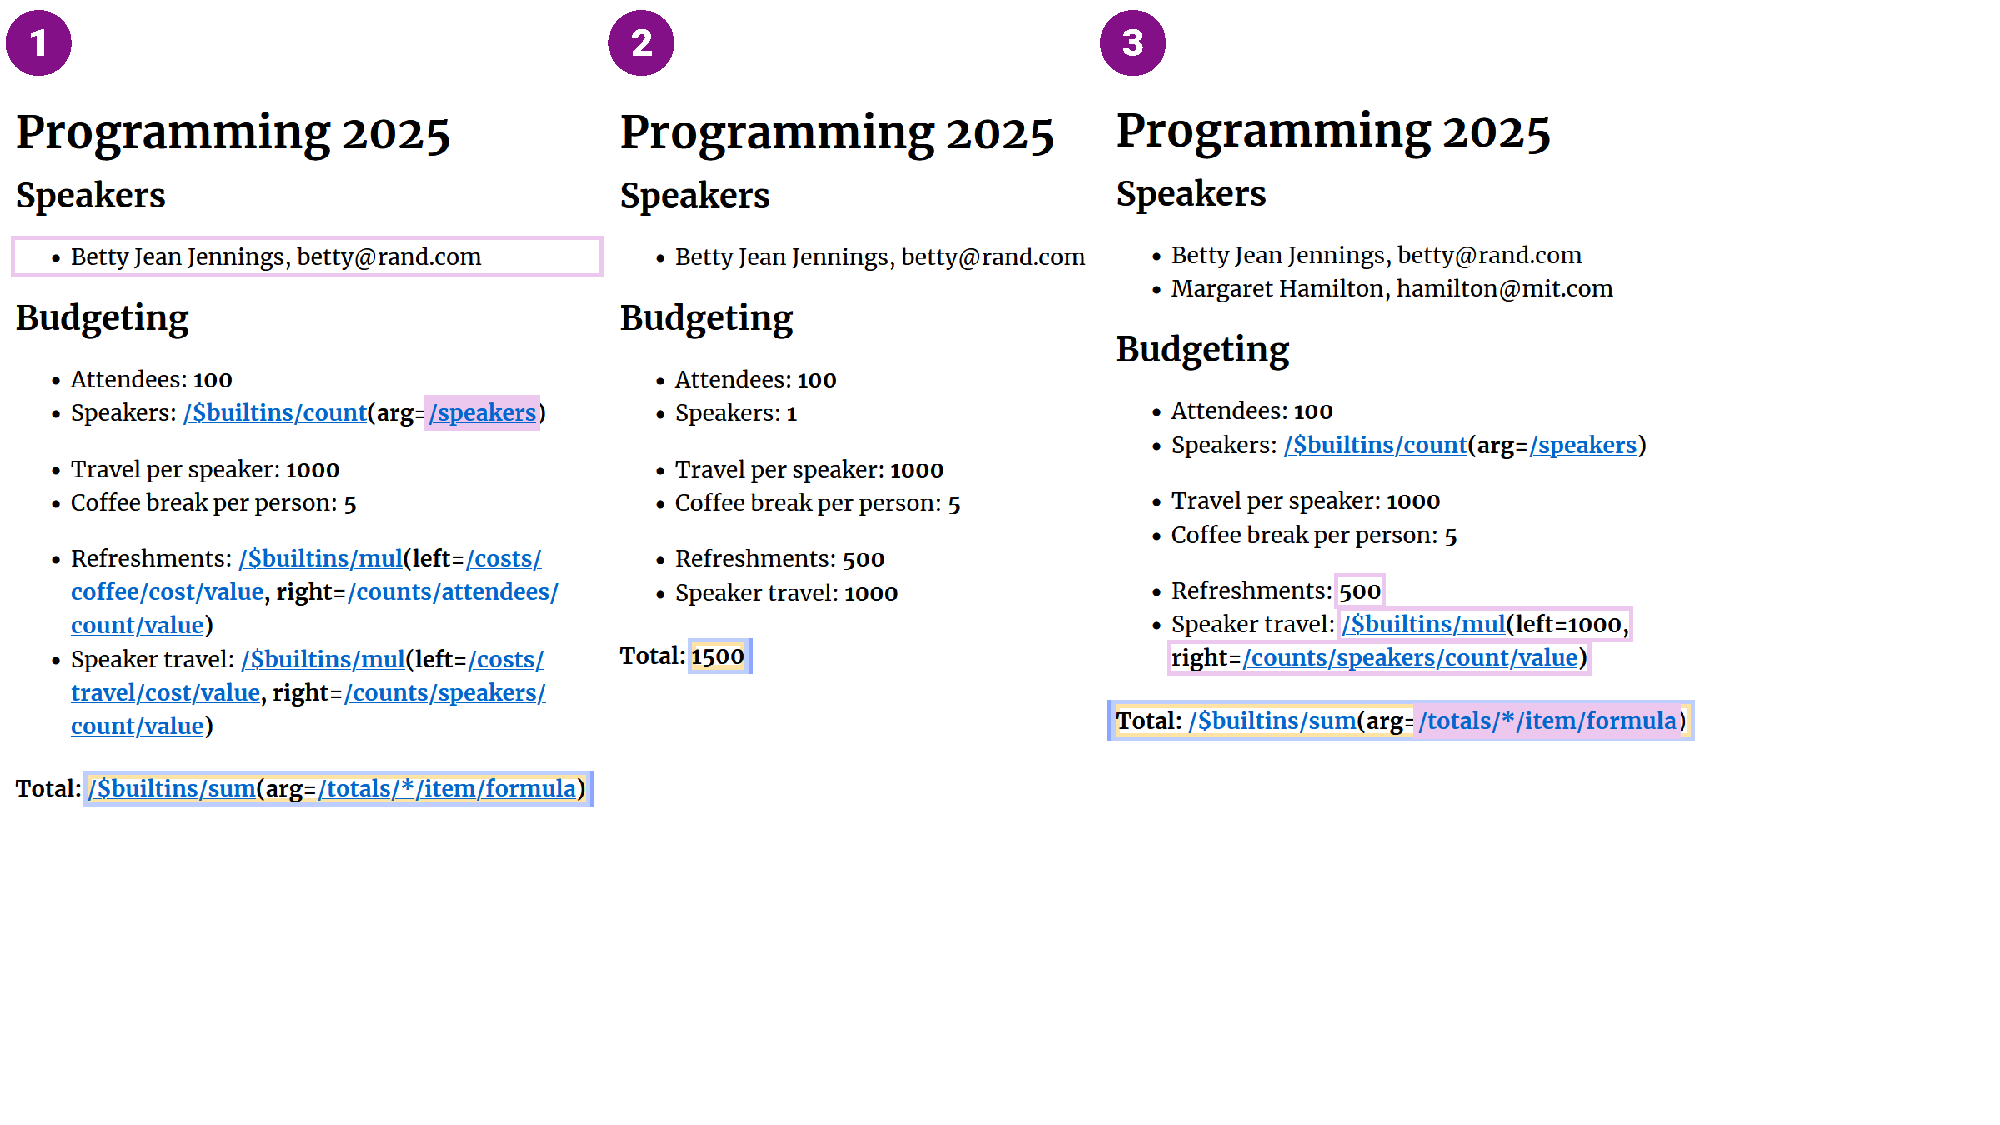
\includegraphics[width=1\columnwidth,clip,trim=0.1cm 5cm 5.1cm 0cm]{fig/incremental.pdf}
  \vspace{-1em}
  \caption{Budget calculation based on the number of speakers (1) and the result (2). When speaker
  is added (3), only the results of affected formulas are invalidated.}
  \label{fig:incremental}
  \vspace{-1em}
\end{figure}

% --------------------------------------------------------------------------------------------------

\subsection{Schema Change Control}
\label{sec:impl-schema}

Document structure often needs to evolve \cite{burnett-2014-silos}, as illustrated by our
Conference List example where a list is transformed into a table. When this happens,
data and code that depend on the structure of the document need to evolve correspondingly.
The problem is well-known in database systems \cite{rahm-2006-schema} and has recently been
studied in the context of programming systems \cite{edwards-2025-schema}.

Although Denicek does not explicitly track document structure (schema or type), all documents
have an implicit structure and some edits transform this structure. As
discussed in \S\ref{sec:system-ops}, Denicek automatically updates reference nodes in the
document when edits modify the document structure. This enables a form of schema code
co-evolution \cite{edwards-2025-schema}. Formulas embedded in Denicek documents use reference
nodes to refer to both data sources (in the document) and the results of other computations.
Consequently, if the document structure changes, the formulas are automatically updated.

Consider the example in Fig.~\ref{fig:coevolution}. The original list {\small\Verb_<ul>_} is
turned into {\small\Verb_<tbody>_} using \ident{UpdateTag} and wrapped inside {\small\Verb_<table>_}
with a field {\small\Verb_body_} using \ident{WrapRecord}. For the latter, Denicek updates the
reference accordingly turning the original {\small\Verb_/speaker_} reference in the formula
into {\small\Verb_/speaker/body_}.

As noted earier, evaluated edits transform the formula structure (wrapping it in the
{\small\Verb_<x-evaluated>_} record). However, they are marked as non-structural and so
references to formulas are not transformed when the formula is evaluated (otherwise, references
would be updated to point to the original unevaluated formulas).

% --------------------------------------------------------------------------------------------------

\begin{figure}[t]
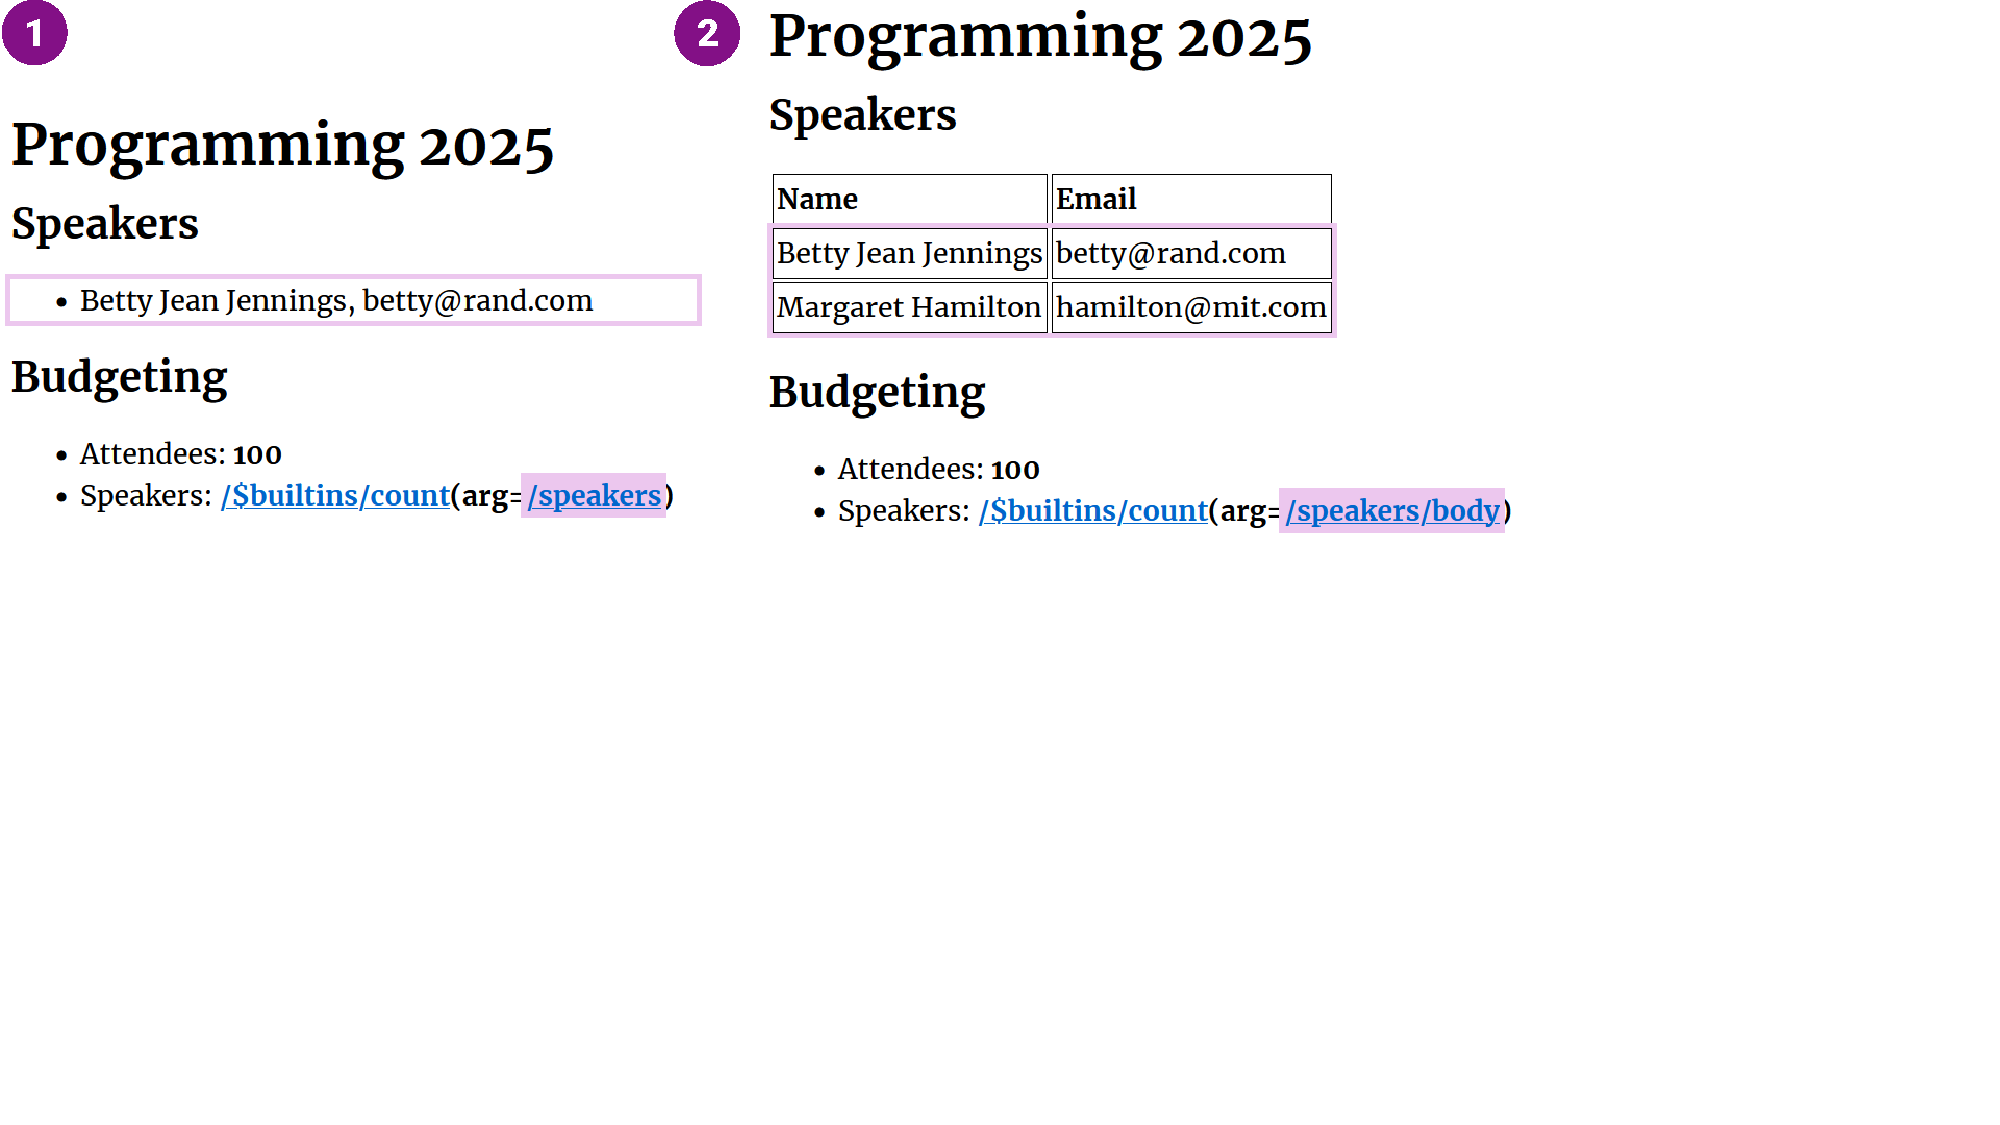
\includegraphics[width=0.9\columnwidth,clip,trim=0cm 9.5cm 8cm 0cm]{fig/coevolution.pdf}
\caption{When an edit changes the document structure, references in formulas are updated accordingly.}
\label{fig:coevolution}
\end{figure}

% --------------------------------------------------------------------------------------------------

\begin{figure}[t]
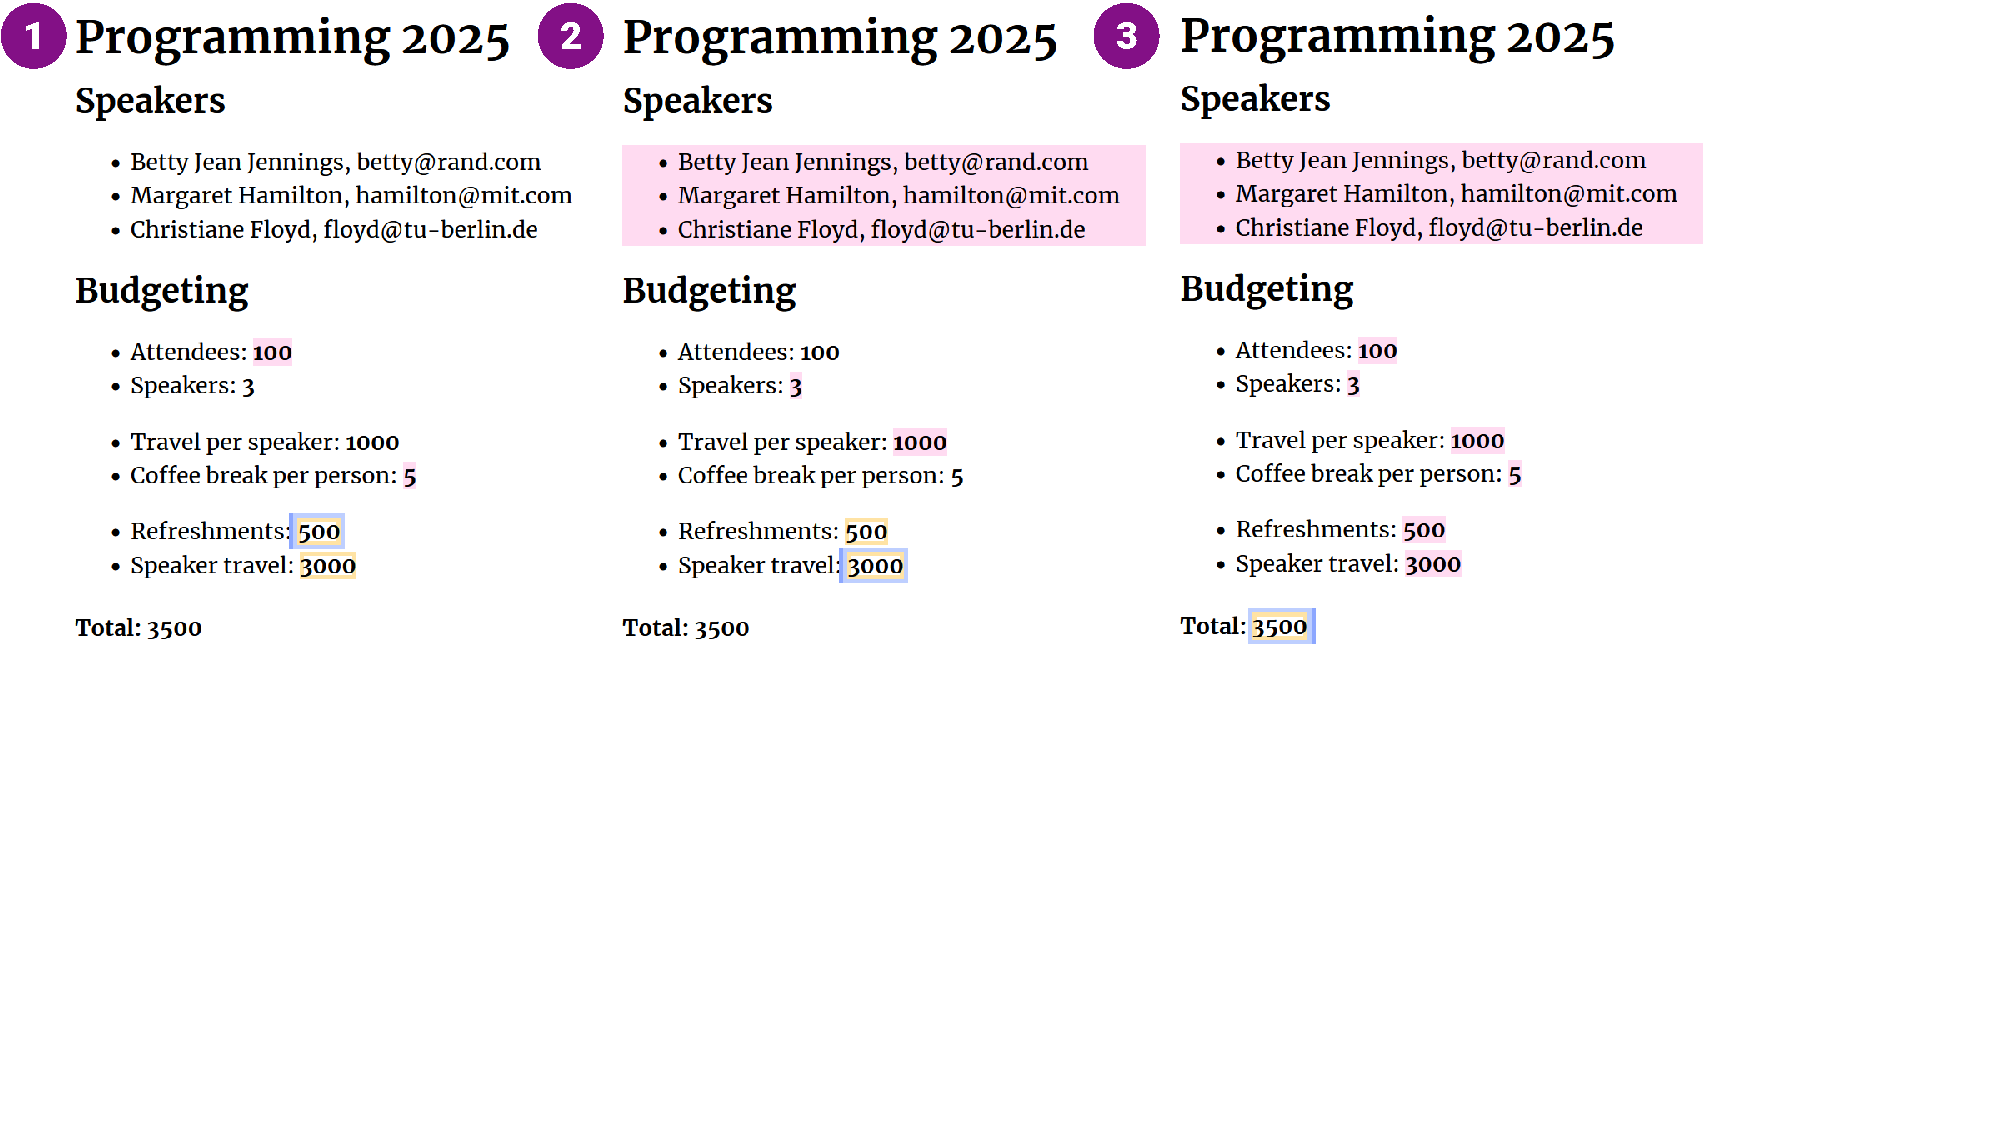
\includegraphics[width=1\columnwidth,clip,trim=0cm 8cm 5cm 0cm]{fig/provenance.pdf}
\vspace{-1em}
\caption{Using provenance tracking to highlight document parts that contributed to the
calculation of refreshments costs (1), travel costs (2) and all costs (3).}
\label{fig:provenance}
\vspace{-0.5em}
\end{figure}

% --------------------------------------------------------------------------------------------------

\subsection{End-User Debugging}
\label{sec:impl-provenance}

The most common kind of end-user programming question is determining whether a value they observe
is right or wrong \cite{kissinger-2006-debugging}. One way to help users answer the question is
to provide an explanation how a value was obtained \cite{ko-2009-whyline}. Webnicek provides a basic
mechanism that highlights document nodes that contributed to a specific computed result,
illustrated in Figure~\ref{fig:provenance}.

The implementation leverages the fact that evaluation keeps the original formula, as discussed
in \S\ref{sec:impl-eval}. When a formula is evaluated, the final {\small\Verb_<x-evaluated>_}
document node contains the result, but also sub-tree that represents a full evaluation trace
\cite{perera-2012-functional}. We analyse the trace, collect all reference nodes in the trace and
highlight all nodes referred to in the computation. Denicek makes this easy as we
only need to collect reference nodes nested in a formula node.

\keyideabox{\faBarChart}{Explanations and Linked Visualizations}{In Webnicek, we implement
provenance analysis to show inputs involved in computation, but information from the execution
trace collected by the Denicek substrate can also be used to provide a detailed
explanation~\cite{perera-2012-functional} or to automatically generate linked visualizations~\cite{perera-2022-linked}.}

% --------------------------------------------------------------------------------------------------

\subsection{Concrete Programming}
\label{sec:impl-copy}

Abstraction is an essential feature of programming, but it has a high cognitive
cost~\cite{blackwell-2002-attention}. Programming by demonstration (\S\ref{sec:impl-pbd})
offers one way of reducing the cost. Another way of making programming more
concrete~\cite{edwards-2004-example,smith-1975-pygmalion} is to support copying of functionality
as in prototype-based object-oriented programming~\cite{randall-1995-self}.

Webnicek supports a functionality akin to managed copy \&
paste~\cite{edwards-2006-copypaste,edwards-2022-copypaste} for formulas. Rather than introducing
abstractions (functions), users can copy and modify formulas to reuse them. However, when the user
discovers an error in the original formula, Webnicek lets them use the merging mechanism to correct
the error in the original formula and all its copies.

The mechanism is shown in Figure~\ref{fig:copypaste}. The user copies an incorrect formula using
the \ident{Copy} edit and then modifies it to use a different data source. They then navigate back
in history to the point before the copying and create a temporary fork of the document. In the
fork, they use \ident{RenameField} to switch the argument of the division. When they merge the
temporary fork into the original document, the \emph{Apply to Newly Added} logic of the merge
operation (\S\ref{sec:system-ops}) duplicates the \ident{RenameField} edits and applies them also
to the copied formula. In other words, the \ident{Copy} edit of the Denicek substrate, alongside
with the fact that formulas are ordinary document nodes, provide keys component for a
straightforward implementation of the managed copy \& paste functionality.

\keyideabox{\faClipboard}{Linked Editing}{Webnicek currently requires users to explicitly
manipulate history to correct error across multiple code clones. Research on managing duplicated
code resulted in multiple tools \cite{toomim-2004-linked,duala-ekoko-2008-clone} with dedicated
user interface to manage clones. The Denicek substrate provides the underlying mechanism that
could be used to implement a more user-friendly interface inspired by those systems.}

% --------------------------------------------------------------------------------------------------

\begin{figure}[t]
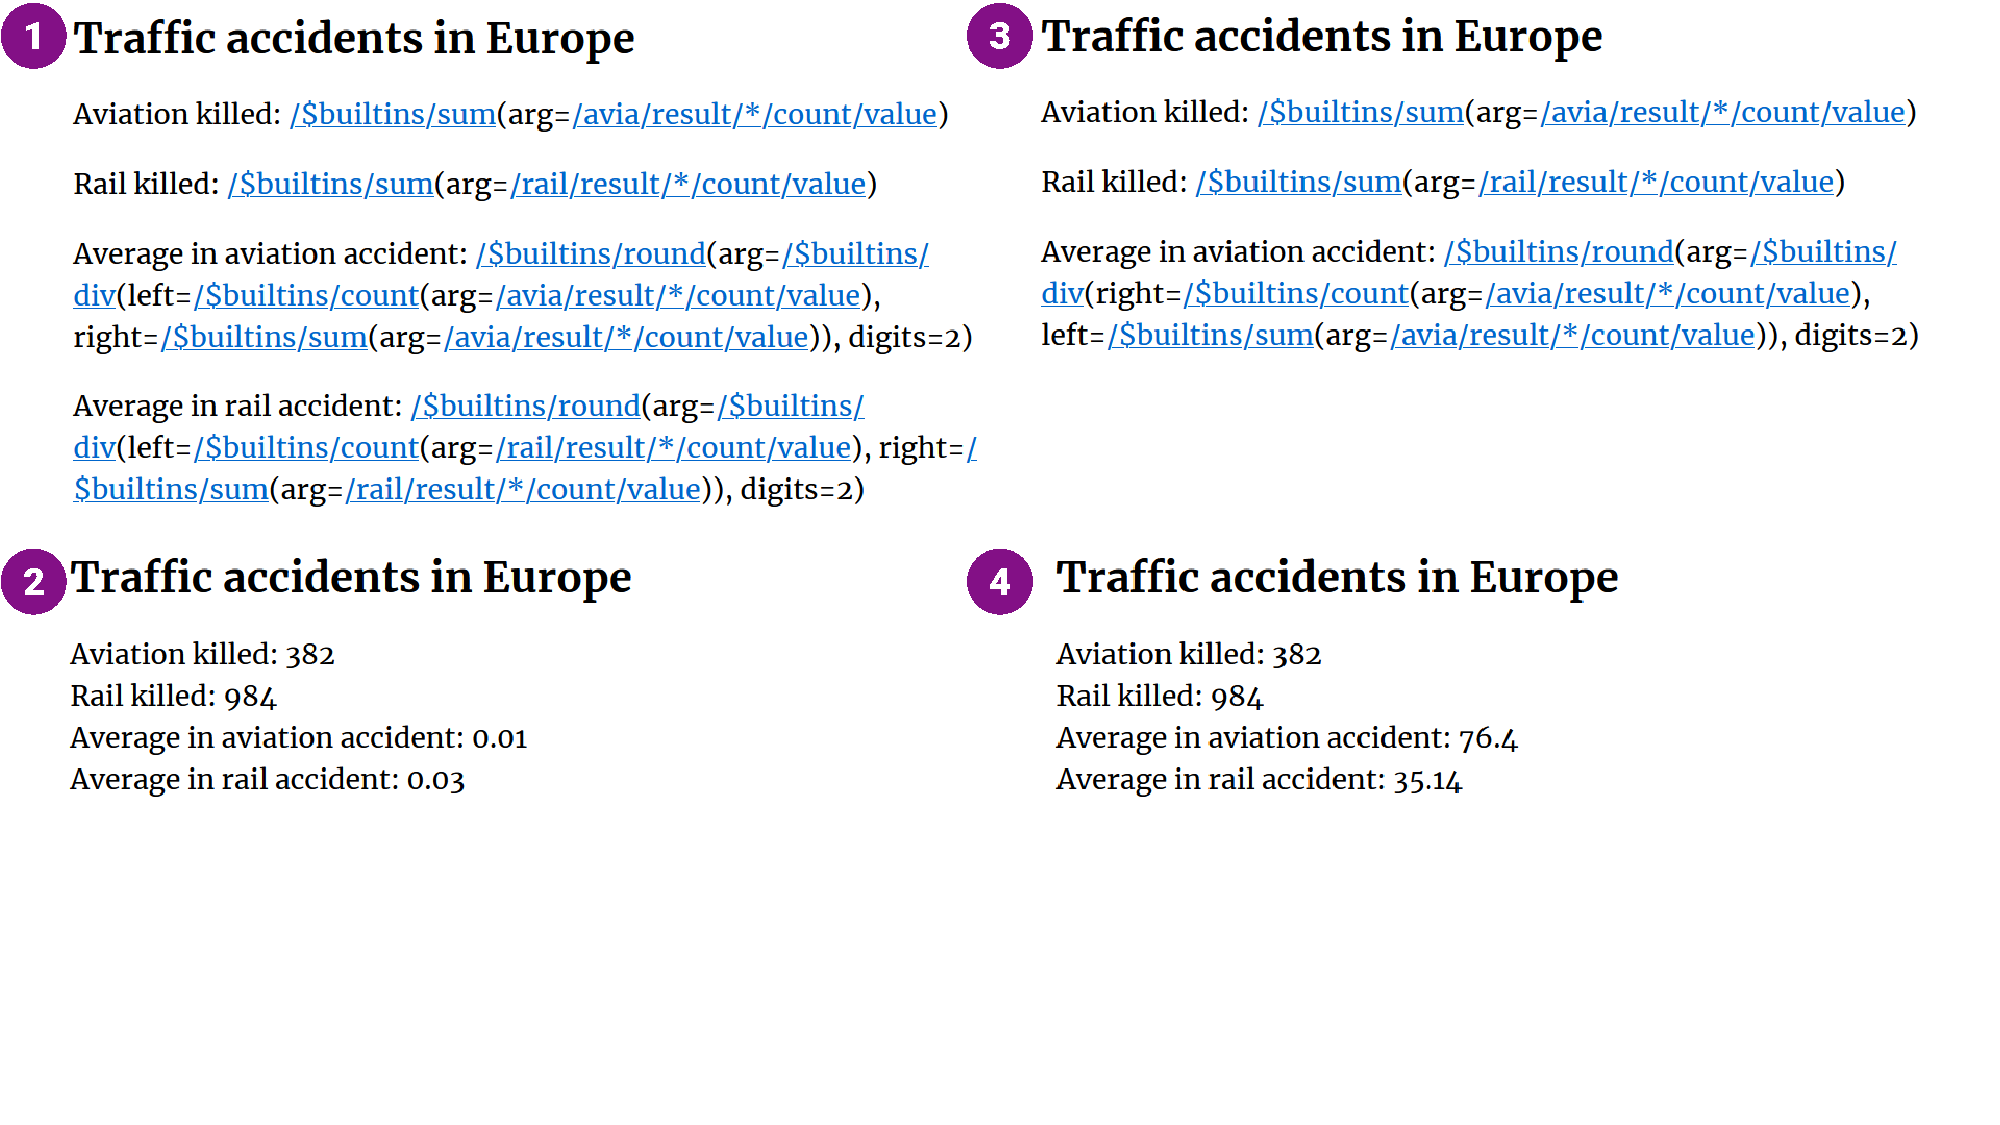
\includegraphics[width=1\columnwidth,clip,trim=0cm 5.5cm 1cm 0cm]{fig/copypaste.pdf}
\vspace{-1.5em}
\caption{Correcting an incorrect formula. The user uses Copy to create the second
formula (1). They notice an error (2), go back in history to switch left and right argument (3),
merge the change and re-evaluate both formulas (4).}
\label{fig:copypaste}
\vspace{-0.5em}
\end{figure}

% ==================================================================================================

\section{Design Considerations}
\label{sec:discuss}

The design of the Denicek substrate is the result of an iterative process in which we repeatedly
adapted the Denicek design until we obtained a satisfactory solution for the six formative examples
(\S\ref{app:examples}) in the Webnicek prototype. In this section, we document the design challenges,
many of which have until now been personal knowledge of researchers working on related
systems \cite{jakubovic-2022-ladder,edwards-2005-subtext,hall-2017-infra,omar-2021-livelits}.

Two guiding principles for Denicek have been \emph{composability} and
\emph{uniformity}~\cite{jakubovic-2023-techdims}. The design should cover a large number of
cases using a small number of concepts. This is apparent in the design of the document
structure (a node can represent data, code or rich text) as well as in the role of edits
(an edit can be a value or structure change, the result of user interaction or the
result of evaluation).

The inconvenience associated with composability and uniformity~\cite{jakubovic-2023-techdims} is not
a problem for Denicek. We view Denicek as an underlying structure on top of which more
convenient end-user programming systems can be built. The uniform design offers a degree of open-endedness,
making it possible to use the basic structures of Denicek in new ways, not anticipated in this paper.

\subsubsection*{Implicit vs. Explicit Structure}
A key design choice for a substrate like Denicek is whether to track the document structure
explicitly or make it implicit. In Denicek, we assume that elements of a list node have the same
structure (i.e.~records should have the same fields, so that they can be targetted using the \ident{All}
selector), but we do not enforce this. Often, the property is temporarily violated when adding a
list item, but then restored once the item is created.

Keeping the structure (type information) explicit has theoretical appeal and it simplifies some
aspects of the implementation. In particular, edits to document structure can be clearly separated
from edits of document values. The same separation has disadvantages in that it complicates the
edit language and it requires user interface that departs further from document editor.
(In Webnicek, users can select all list items and edit them at once using the same mechanism as
when editing individual list items. With explicit structure, changing a list structure has to be
either a different kind of edit or possibly an edit of a virtual ``prototype'' element.)

\subsubsection*{Merging and Document State}
One specific design choice in Denicek is that the merge operation operates solely on two
sequences of edits, but it does not need access to the current document state (or full edit
histories). The reconcilliation of edits (\S\ref{sec:system-ops}) is defined for two individual
edits $e_1$ and $e_2$.

This design limits the possible language of edits. We cannot, in general, support
conditional edits (that are applied only when a certain condition holds for
the current document state). This is because the merging operation would not be able to
determine whether the edit is applied (and whether its effects should~take~place).

One consequence of the design choice is that the generalization of recorded interactions (\S\ref{sec:impl-interaction}) has to
be done on a meta-level (by specifying how to invoke edits, rather than through the edits themselves).
Another consequence is that our langauge of selectors has to be abstract.
We can target all list elements using the \ident{All} selector, but cannot combine this
representation with a representation that explicitly lists indices of all items currently in the list.

\subsubsection*{Explicit List Indices}
Denicek does not use implicit numerical indices for lists. When adding an item, the
user (or the system built on top of Denicek) has to explicitly provide an index. This design
is motivated by a typical programming by demonstration scenario where the user adds a
new list item and then modifies it (adding a speaker or a Todo item). When using explicit indices,
the edits following \ident{Append} can use the index to refer to and modify the newly added
item. (To avoid overwriting existing items when replaying recorded edits, Webnicek replaces
indices of newly added items when replaying recorded interactions in \S\ref{sec:impl-pbd}).

Using implicit numerical indices is possible, but it requires treating all list-related edits
as operations that transform document selectors. This means adding multiple new rules to
Figure~\ref{fig:updates}, which specifies how edits transform references. Merging then has to
modify indices when edits add, remove or reorder list items. List order then, somewhat confusingly,
becomes a part of document structure rather than a property of the list value.

The problem could be avoided by not letting the user modify a list item after adding it.
(We can require new items to be constructed outside of the list and then added through a
single edit that combines the logic of \ident{Append} and \ident{Copy}.) This is easy to
implement, but it requires unintuitive user interaction and it also does not address all
use cases for modifying list item via index.

\subsubsection*{Ordering List Items and Record Fields}
When list indices are not numerical and supplied explicitly, we need another mechanism for
tracking order of list items. Denicek uses a data structure inspired by Mergeable Replicated
Data Types \cite{kaki-2019-mrdts} and requires specifying the index of a preceding list item
when appending to a list. However, Webnicek supplies the index of preceding item automatically.
(If two edits append to the same list independently with the same preceding item, the order
is non-deterministic.)

Note that Denicek uses the same mechanism for record fields. Keeping record fields ordered is
desirable because Denicek documents map directly to HTML documents and so the order is visible
to a user. Moreover, different ways of merging edits can result in different order of adding fields
to a record. Making order explicit ensures those result in equivalent documents.

Denicek still makes a distinction between records and lists, even if the two are similar
technically. The difference is conceptual. A list is expected to contain items of the
same structure (that can be addressed using the \ident{All} selector), whereas record fields
are expected to be of different types. If we unified lists and records, \ident{All} would have
to be applicable to records too and inferring and checking document structure would be
challenging.

\subsubsection*{Convergence vs. Divergence of Document Variants}
There are two ways of managing document variants in collaborative editing~\cite{edwards-2025-schema}.
In the \emph{divergence} model, users can maintain their own variant indefinitely (share data,
but use a different schema locally). In the \emph{convergence} model, users have to adopt all
earlier changes in order to adopt a later change (accept new schema before new data).

Denicek supports only the simpler \emph{convergence} model. To support the \emph{divergence}
model, we would need an operation dual to our edit reconcilliation (given two subsequent edits,
$e_1, e_2$, we want to generate $e_2'$ that has the same effect as $e_2$ but can occur before
$e_1$). The pair of operations has been called \emph{project} and \emph{retract}
\cite{edwards-2021-typed}. We choose not to support this as it would complicate the basic
Denicek substrate structure.

\subsubsection*{Linear History vs. Graph of Edits}
Denicek keeps a linear history of edits. When merging edits, new edits have to be transformed and
added to the top of the history. This model is akin to git rebase. An alternative representation
would be to maintain a graph of edits akin to when using git merge. In this representation,
we would need to keep parents of edits and special merge edits would have multiple parents.

Maintaining a graph of edits would make recording of edits in programming by demonstration
easier (\S\ref{sec:impl-pbd}) as we would not need to update recorded edits if they are
transformed during merging. (Their hashes would remain the same.) However, supporting special
merge edits and non-linear history would make the basic substrate more complex.

\subsubsection*{Supporting Rich Selectors}
Denicek supports only a limited set of selectors. An absolute reference can select a record
field (\ident{Field}), specific list item (\ident{Index}) or all list items (\ident{All}).
Once can imagine a range of other useful selectors, for example to select list items with a
given tag or select items satisfying other conditions.

We could support such selectors for those edits that do not affect the document
structure. However, supporting such conditional selectors in general is incompatible with our
design decision that merging should not depend on document state. (If an edit wraps the body of all
{\small\Verb_<h3>_} elements, we need to know the document state in order to determine whether
we need to modify the selector pointing to an item at a specific index.)

\subsubsection*{Dependency Tracking}
Recall that the incremental recomputation (\S\ref{sec:impl-incremental}) is based on the
conflict detection mechanism of Denicek (\S\ref{sec:system-ops}). When pushing edit $e_2$ through
$e_1$, a conflict is detected if they affect overlapping targets or if $e_1$ modifies a
document node that is a source of $e_2$, typically, the source of a \ident{Copy} edit.

For edits generated during formula evaluation (\S\ref{sec:impl-eval}), we need to track an
additional kind of dependency. Evaluating a formula that adds two numbers from two document
location results in an edit that sets the result of the formula to the sum of the two numbers.
The edit contains the resulting number, but we also need to record that the edit has the two
source locations as dependencies. For this reason, Denicek makes it possible to annotate edits
with additional dependencies. One alternative would be to introduce a special \ident{Evaluate}
edit that would identify an operation to compute and a list of arguments, specified as a list
of references. We choose the former to keep the set of edits smaller.


% ---------------------------------

\begin{comment}
Maybe have 'enabled' for edits afterall?
(we can merge with conflicts and disable some edits, but keep them in history for info)


TODO - things to work on
* "represent" edits somewhere in document as "library of functions"
  and then call those from buttons (rather than embedding them directly)
  allow some kind of abstraction (as in Histogram) to make them reusable
* figure out how to do evaluation better
  (based on the stored abstractions? but need to store provenance...)

SEMANTIC CONDITIONS
\url{https://www.youtube.com/watch?v=NBnc2ToS_j0}
(has a section on this in background)



INTERACTION
* replay stored event handlers against the old version?
  (this way, adding an item to a speakers list gets migrated \& adds a new table row!)
* simlarly!! we need merge in order to apply edits to multiple targets
  (when you remove all items in a list, the indices change)
  (but I guess we should do this against version at the time of saving too....)

[this \& evaluation = the unreasonable effectiveness of merging]

Notes on storing and reusing edits
* references need to be represented as references so that they get updated
  (NO! not if we reply them against old version, which seems better - but there are 2 design choices)
* how to apply them to multiple targets? use Move to update the selectors instead of
  replacing the prefix manually


CONDITIONALS
https://toby.li/files/p311-radensky.pdf

\end{comment}

\subsection{Future work}
\label{sec:discuss-future}
Although Denicek does not explicitly track document structure (or schema, or type), all documents
have an implicit structure.
=> use type system to check temporarily invalid state

better effect system

IDEA: Type check edit groups to ensure they preserve structure but not individual edits eg when adding list item

~

~

~

% memory mapped graphics etc.





\section{Case study}
\label{sec:case}
(data science environment)

\section{Evaluation}
\label{sec:eval}
how well did Denicek work for implementing Datnicek

\section{Discussion}


\begin{comment}


\subsection{Heuristic evaluation}

techdims

\subsection{Limitations}

RANDOM FORMAL STUFF

ohter formal things
* non-conditionality of edits
* show that they can transform document from any to any without removing/readding values


PROPERTIES
- can change any document to any other - sure, via remove add - but also more semantically
(if it contained all values, can we do it without removing and adding them?)

DEMOS

// cf shadow dom v reactu
// something like google forms!

* two ways of pushing edits should be equivalent, i.e.

push e1 e2 e3 over b1 b2 b3 can be done via
  push e1 over b1 = e1'; over b2 = e1''; over b3 = e1'''
  then push e2, then push e3
or
  push e1, e2, e3 over b1, then over b2, then over b3
(implies that no "extra" edits can be appended later)
\end{comment}

\bibliographystyle{plain}
\bibliography{paper}


\newpage
~
\newpage



\appendix
\section{Formative Examples}
\label{app:examples}

The design the Denicek substrate, we identified six formative examples shown in
Fig.~\ref{fig:examples}. The examples range from established industry benchmarks
(Todo and Counter apps) to cases from literature~\cite{edwards-2022-copypaste} and
problems posed as schema change challenges \cite{edwards-2025-schema}.
The Denicek substrate then co-evolved with Webnicek, a simple web-based programming environment
built (as directly as possible) on top of the substrate and was used to solve implement the
formative examples.

Many of the formative examples include a small programming challenge, such as adding
user interface to add a new speaker, a new list item or modify the count. Our aim was for
the substrate to enable solving  those through programming by demonstration.
Programming by Demonstration is often used in data wrangling
\cite{gulwani-2012-spreadsheet,drossos-2020-wrex,gulwani-2014-flash}. Our Hello World example
is only a minimalistic illustration of such use, loosely inspired by earlier work \cite{miller-2001-simult}.

\section{Merging Edit Histories}
Recall that merging takes two edit histories, $E, E_1$ and $E, E_2$,
transforms edits $E_2$ into $E_2'$ that can be reapplied on top of the first history
resulting in $E, E_1, E_2'$. The key operation takes two individual edits, $e_1$ and $e_2$
and produces a sequence of edits $e_2', e_2'', \ldots$ that can be applied after $e_1$,
and combine the two edits. This section provides details about the two aspects of this operation.

\subsection{Apply to Newly Added}
\label{app:merge-apply-to-added}

Assume that edits $e_1$ and $e_2$ occurred independently. We want to modify $e_2$ so that
it can be placed after $e_1$. If the edit $e_2$ added new nodes to the document that the
edit $e_1$ would affect, we generate an additional edit that apply the transformation of $e_1$
to the newly added nodes (and only to those).

The only edits that add new document nodes are \ident{Add}, \ident{Append}, \ident{Copy} and
so we consider this case if the edit $e_2$ is one of those. If so, we check
whether the target of $e_1$ is within the target of $e_2$, i.e., the list of selectors that
forms the target of $e_2$ is a prefix of the list of selectors that forms the target of $e_1$.

Along the way, we compute a \emph{more specific prefix}. If the target of $e_1$ contains
the \ident{All} selector, it can be matched against a specific \ident{Index} selector in the
target of $e_2$ (if the selector of $e_1$ is more specific than that of $e_2$, the targets
are not matched). We then replace the original prefix in $e_1$ with the \emph{more specific prefix}
that contains \ident{Index} selector in places where the original edit contained \ident{All}.
This way, we obtain $e_1'$ which is a focused version of $e_1$ that applies only to the
nodes newly added by $e_2$. The edit $e_2$ thus becomes a pair of edits $e_2, e_1'$.
The final document will contain edits $e_1, e_2, e_1'$ -- that is, it will first apply the edit
$e_1$ to nodes already in the document, then add new nodes and then apply the transformation
represented by $e_1$ to the newly added nodes.

\subsection{Transform Matching References}
\label{app:merge-transform-refs}

As above, assume that edits $e_1$ and $e_2$ occurred independently. We want to
modify $e_2$ so that it can be placed after $e_1$. If $e_1$ is any of the three edits
listed in Fig.~\ref{fig:updates} (\ident{RenameField}, \ident{WrapRecord}, \ident{WrapList}),
we collect all references that appear inside $e_2$ (the target, the source of \ident{Copy}
and any references occurring in the nodes added by \ident{Add} or \ident{Append}).
If the target of $e_1$ is a prefix of any of those references, we update the references
accordingly and obtain a new edit $e_2'$. Note that it would be an error to match specific
\ident{Index} in $e_1$ with more general \ident{All} in $e_2$, but this cannot happen --
reference updating is not done when the target of $e_1$ contains \ident{Index}.

Now consider the case when $e_1$ is \ident{Copy} and the edit $e_2$ targets a node that is
the source node of the copy operation (or any of its children). In this case, it is reasonable
to require that the edit $e_2$ is applied to both the source and the target of the copy.
(This is required by the refactoring done in the Conference Budget example.)
We handle the case by creating a copy of $e_2$ with transformed selectors (target and, if $e_2$
is also \ident{Copy}, also its source). To transform the selectors, we replace the prefix
formed by the source of the \ident{Copy} by a new prefix, formed by the target target of
the \ident{Copy}. We then add the new operation as $e_2'$ if at least one of its selectors
was transformed (typically target, but possibly also source).

\begin{figure}
\newcommand{\extablecol}[5]{
\small{\bfseries #1} #2\,\; --\,\; #3\\[-0.1em]
\quad \footnotesize #4 \\[-0.2em]
\quad \footnotesize \emph{#5} \\[0.4em]
}

\begin{tabular}{|l|}
\hline
\\[-1em]
\extablecol{Counter App}{\cite{kiss-2014-7guis}}
  {Counter with increment and decrement buttons.}
  {The current count is represented by a formula that is modified by the buttons.\\[-0.2em]\quad\footnotesize
  The user can inspect the evaluation trace to see how the count was modified.}
  {Programming by Demonstration, Incremental Recomputation, End-User Debugging}
\extablecol{Todo App}{\cite{osmani-2024-todomvc}}
  {Buttons to add an item and remove all completed.}
  {Adding an item must correctly merge with independently added functionality to \\[-0.2em]\quad\footnotesize
   compute which items are completed and remove them based on a formula result.}
  {Programming by Demonstration, Local-First Collaboration, Incremental Recomputation}
\extablecol{Conference List}{\cite{edwards-2025-schema}}
  {Manage a list of invited conference speakers.}
  {Adding speakers to a list through an in-document user interface merges with \\[-0.2em]\quad\footnotesize
   refactoring that turns the list into a table and separates name from an email.}
  {Local-First Collaboration, Programming by Demonstration}
\extablecol{Conference Budget}{\cite{edwards-2025-schema}}
  {Calculate budget based on a speaker list.}
  {References are updated  when the list is refactored. Only affected formulas\\[-0.2em]\quad\footnotesize
   are recomputed and the user can view elements on which the result depends.}
  {Local-First Collaboration, Incremental Recomputation, End-User Debugging}
\extablecol{Hello World}{\cite{miller-2001-simult}}
  {Normalize the capitalization of two word messages.}
  {An operation to normalize the text in a list item can be recorded and applied to\\[-0.2em]\quad\footnotesize
   all list items or, alternatively, applied directly to all list items.}
  {Programming by Demonstration}
\extablecol{Traffic Accidents}{\cite{edwards-2022-copypaste}}
  {Compute statistics using two data sources.}
  {Formula to compute statistics can be reused with a different data source;\\[-0.2em]\quad\footnotesize
   error correction is propagated automtically to the copied version of the formula.}
  {Concrete Programming, Incremental Recomputation}
\hline
\end{tabular}

\caption{Formative examples used in Denicek design}
\label{fig:examples}
\vspace{-1em}
\end{figure}

NICE THINGS IN DATNICEK
* merging of code edits (e.g. change parameter merges with adding a call to chain)
* remove cell to which there are refs - does the susbtrate catch this?

RELATED WORK

TIJS
https://homepages.cwi.nl/~storm/publications/icsews13live-p17-p-16201-preprint.pdf

via Pierre
https://pijul.org/manual/why_pijul.html

Geoffrey Litt
https://dl.acm.org/doi/pdf/10.1145/3426428.3426914
https://dl.acm.org/doi/pdf/10.1145/3397537.3397541

Programming By Example: Intelligence in Demonstrational Interfaces
https://cacm.acm.org/research/programming-by-example-intelligence-in-demonstrational-interfaces/

Rapido: Prototyping Interactive AR Experiences through
Programming by Demonstration
https://dl.acm.org/doi/pdf/10.1145/3472749.3474774

openrefine
- facet (group by) - then change the key to normalize
  (https://www.youtube.com/watch?v=yTJ6x6zEQmI 51:40)

Don't Step on My Toes: Resolving Editing Conflicts in Real-Time
Collaboration in Computational Notebooks
https://arxiv.org/pdf/2404.04695

AI assistants in notebook interfaces
https://dl.acm.org/doi/pdf/10.1145/3544548.3580940

Unravel - understand pipelines
https://dl.acm.org/doi/pdf/10.1145/3472749.3474744

WREX - nicest tool
https://dl.acm.org/doi/pdf/10.1145/3313831.3376442

\begin{comment}
\newpage
xx

~\\
introduction \\
background \\
related work \\
design process / goals \\
case study \\
formative research \\
formative study \\
analysis \\
system \\
implementation \\
evaluation / heuristic evaluation \\
discussion and limitations \\

\newpage
\section{Introduction old}

The computational substrate using which software is built determines the capabilities that the
software can provide. An imperative substrate that views programs as instructions modifying
bytes in memory makes it almost impossible to allow end-user inspection or reprogramming of
running software.

substrate as defined by \cite{jakubovic-2022-ladder}


A computational substrate defines what software is built from. This may be objects as in
Smalltalk, lists as in Lisp, or memory with data and code as in UNIX/C.
The different substrates enable different kinds of programming experiences.
For example, object-oriented programming has historically been linked to the development
of graphical user interfaces (where objects can correspond to elements on the screen).
It has also enabled the development of visual programming environments such as the Alternate
Reality Kit, based on message sending between objects.

In principle, any computational substrate can be used to develop any programming experience,
but the greater the impedance mismatch between the substrate and the desired experience,
the more difficult it will be to provide the experience and combine it with the rest of the
system and other programming experiences developed for the system. (One can implement support
for programming-by-demonstration using C/C++, for example as part of a game scripting engine,
but it will not work with the rest of the ordinary C/C++ ecosystem.)


Medium is the message

\subsection{Substrate}

The question asked in this paper is, what would be the ideal programming substrate
for supporting a range of programming experiences that make programs more
collaborative, transparent and allows for a gradual transition from non-programmer
to a programmer. We want a programming substrate that makes it easy to develop
programming experiences such as:

\begin{itemize}
\item \emph{Programming by demonstration} --
  Allow non-programmers to construct simple programs by performing examples of the expected behaviour. \cite{leiva-2021-rapido}.
\item \emph{Local-first collaboration} --
  Multiple users should be able to use and modify a single program, preferrably without requiring a central server. \cite{kleppmann-2019-local}
\item \emph{Provenance tracking} --
  The execution of the program should leave an understandable trace that lets the user understand why program resulted in a particular result.
\item \emph{Schema evolution [extra-ish]} --
  When the user evolves the structure of the program, data and code should co-evolve automatically to match the new structure.
\item \emph{Notational freedom [extra-ish?]} --
  Allow users to adapt the program using a notation that suits them and is appropriate for the programming task at hand. [Joel]
\item \emph{Concrete programming [extra?]} --
  It should be possible to reuse parts of program or program logic without constructing abstractions, for example by managed copy \& paste.\cite{edwards-2006-copypaste,edwards-2022-copypaste}
\end{itemize}

substrate as defined by \cite{jakubovic-2022-ladder}

% pbd
\cite{leiva-2021-rapido,cypher-1993-pbd}
\cite{chen-2023-miwa}

% lcoal first
\cite{kleppmann-2019-local,klokmose-2024-mywebstrates}
% provenance
\cite{ko-2004-whyline,ko-2009-whyline,krebs-2023-probelog}
\cite{ricciotti-2017-imperative,perera-2012-functional}
\cite{perera-2022-linked}


% visualizations of results or execution
% https://www.dcs.warwick.ac.uk/pvw04/p01.pdf
% https://dl.acm.org/doi/10.1145/3313831.3376494

% previews - livelits

% Schema evolution
% our paper; see https://openproceedings.org/2023/conf/edbt/paper-160.pdf - good refs in 2.2

% https://x.com/jonathoda/status/1185888711210389504

% also cool: https://arxiv.org/pdf/2303.06777

% Hazel family of things
% structure editing - sandblocks

Joel's definition of substrate in Onward!
Bret Victor talk
\url{https://www.youtube.com/watch?v=ef2jpjTEB5U}

In what ways is a substrate "natural"?

thinglab - create line by cloning, it sticks to mouse pointer, clicking sticks it to something else
squeak - has all the browsers (method search...)


computational substrate
how it differs from computational media?
more low-level - media suggests that there it comes

\section{The whatever system}
\subsection{Document + Edits}
defines
\begin{itemize}
  \item selectors
  \item nodes
  \item edits
\end{itemize}

\subsection{Walkthrough}
* todo list? (or counter, but that is a bit boring)

\section{Themes}
* programming by demonstration
  - binding interactions to gui elements (event handlers)
* provenance tracking
  - Amy Ko's whyline, Probe Log by HPI, enables linked visualizations
* merging of edit histories / collaborative editing
  - bonus - can share restricted link to allow users fill out
    forms (allow partial edits only / def by selector?)
* scehma change - change data \& code accordingly
* everything is an edit
  - interaction with the GUI
  - evaluation? tbd
* copy \& paste abstraction
    (requires finishing new approach to formulas!)
  - edit before copy to propagate edit to other places
    (or edit after copy to make it specific to a case)
  - higher order copying from https://tomasp.net/academic/papers/copy-paste/paint22.pdf
* augmenters
  - cf. bonnie nardi (calls them something else - Jonathan says)
  - add programming by demonstration data wrangling gui to table (trigger interactions)
    cf. lorgnette

\section{Applications}
* todo list / counter / maybe too simple
* (if used in the walkthrough, maybe something else? board game as in varv - tic tac toe? or 7guis?)
* conference organizer
* data exploration (ala histogram)
* linked charts

\section{Extras}
* metablocks?
* self-sustainability
* some non-browser implementation of this (as in Varv?)

explicit structure
self-sustainability
notational freedom

\newpage
~

REMAINING IMPLEMENTATION TODOs:

* Some kind of provenance visualization
* Some kind of matchers/transformers mechanism (ideally to add interactive buttons to tables)
* Apply to all (remove completed in TODO)

\newpage
~


append /speakers \#hamilton <li>
addfld /speakers/\#hamilton speaker "Margaret Hamilton, hamilton@mit.edu"

>>> wraprec /speakers body <table>

[update selectors - add /body]
append /speakers/body \#hamilton <li>
[dtto]
addfld /speakers/body\#hamilton speaker "Margaret Hamilton, hamilton@mit.edu"

>>> retag /spekers/body <tbody>

[na - out of scope]

>>> retag /speakers/body/* <tr>

[apply to added - update node (* => \#hamilton scoping)]
append /speakers/body \#hamilton <li>
+ retag /speakers/body/\#hamilton <tr>
[na - out of scope]
addfld /speakers/body\#hamilton speaker "Margaret Hamilton, hamilton@mit.edu"

>>> wraprec /speakers/body/*/speaker value <td>

append /speakers/body \#hamilton <li>
+ retag /speakers/body/\#hamilton <tr>
+ wraprec /speakers/body/\#hamilton/speaker value <td> [ no op - it is not there]
addfld /speakers/body/\#hamilton speaker "Margaret Hamilton, hamilton@mit.edu"
+ wraprec /speakers/body/\#hamilton/speaker value <td>

>> updid /speakers/body/* speaker=>name

append /speakers/body \#hamilton <li>
+ retag /speakers/body/\#hamilton <tr>
+ wraprec /speakers/body/\#hamilton/speaker value <td> [ no op - it is not there]
+ updid /speakers/body/\#hamilton speaker=>name [ no op - it is not there ]
addfld /speakers/body \#hamilton speaker "Margaret Hamilton, hamilton@mit.edu"
+ wraprec /speakers/body/\#hamilton/speaker value <td>
+ updid /speakers/body/\#hamilton speaker=>name

>>> addfld /speakers/body/* email ""

append /speakers/body \#hamilton <li>
+ retag /speakers/body/\#hamilton <tr>
+ wraprec /speakers/body/\#hamilton/speaker value <td> [ no op - it is not there]
+ updid /speakers/body/\#hamilton speaker=>name [ no op - it is not there ]
+ addfld /speakers/body/\#hamilton email "" [ no op - it is not there ]
addfld /speakers/body \#hamilton speaker "Margaret Hamilton, hamilton@mit.edu"
+ wraprec /speakers/body/\#hamilton/speaker value <td>
+ updid /speakers/body/\#hamilton speaker=>name
+ addfld /speakers/body/\#hamilton email ""

...

copy /speakers/body/*/name => /speakers/body/*/email
edit /speakers/body/*/name (fn1)
edit /speakers/body/*/email (fn2)











\end{comment}



















\end{document}
